%%%%%%%%%%%%%%%%%%%%%%
\documentclass{amsart}
% !TEX root = ../ac_paper.tex

% General packages
\usepackage{microtype}
\usepackage{amsmath, amssymb, amsthm}
\usepackage{mathtools}
\usepackage{tikz-cd}
\usepackage{mathbbol} % changes \mathbb{} and adds more support

% Complex configurations
% bibliography
\usepackage[
backend=biber,
style=alphabetic,
backref=true,
url=false,
doi=false,
isbn=false,
eprint=false]{biblatex}

\renewbibmacro{in:}{} % don't display "in:" before the journal name
\AtEveryBibitem{\clearfield{pages}} % don't show page numbers

\DeclareFieldFormat{title}{\myhref{\mkbibemph{#1}}}
\DeclareFieldFormat
[article,inbook,incollection,inproceedings,patent,thesis,unpublished]
{title}{\myhref{\mkbibquote{#1\isdot}}}

\newcommand{\doiorurl}{%
	\iffieldundef{url}
	{\iffieldundef{eprint}
		{}
		{http://arxiv.org/abs/\strfield{eprint}}}
	{\strfield{url}}%
}

\newcommand{\myhref}[1]{%
	\ifboolexpr{%
		test {\ifhyperref}
		and
		not test {\iftoggle{bbx:eprint}}
		and
		not test {\iftoggle{bbx:url}}
	}
	{\href{\doiorurl}{#1}}
	{#1}%
}
 % bibliography management
% hyper-references
\usepackage[
bookmarks=true,
linktocpage=true,
bookmarksnumbered=true,
breaklinks=true,
pdfstartview=FitH,
hyperfigures=false,
plainpages=false,
naturalnames=true,
colorlinks=true,
pagebackref=false,
pdfpagelabels]{hyperref}

\hypersetup{
	colorlinks,
	citecolor=blue,
	filecolor=blue,
	linkcolor=blue,
	urlcolor=blue
}

% cross-references
\usepackage[capitalize, noabbrev]{cleveref} % hyper- and cross-referencing 

% Update to MSC2020
\makeatletter
\@namedef{subjclassname@2020}{%
	\textup{2020} Mathematics Subject Classification}
\makeatother

% Table of contents
\setcounter{tocdepth}{2}
\input{aux/usualcmds}

%%%%%%%%%%%%%%%%%%%%%%
% !TEX root = ../template.tex

% Include adittional packages below
\usepackage{amsfonts}
\usepackage{graphicx}
\usepackage{xcolor}
\usepackage{enumitem}
\usepackage{caption}
\usepackage{subcaption}
\usepackage{algorithm}
\usepackage{algpseudocode} % new packages here
% !TEX root = ../template.tex

\newcommand{\bea}{\begin{eqnarray}}
\newcommand{\eea}{\end{eqnarray}}
\newcommand{\fixme}[1]{{{\color{blue}{[#1]}}}}
\newcommand{\AK}{\text{AK}}
\newcommand{\MS}{\text{MS}}
\newcommand{\G}{\text{G}}
\newcommand{\C}{\mathbb C}
 % new commands here
\addbibresource{aux/bibliography.bib} % new references here

%%%%%%%%%%%%%%%%%%%%%%
\title[What makes math problems hard for RL]{What makes math problems hard for reinforcement learning: a case study}
% !TEX root = ../ac_paper.tex

\author{A.~Shehper}
\address{NHETC, Department of Physics and Astronomy, Rutgers University, Piscataway, New Jersey 08854, USA}

\author{A.~Medina-Mardones}
\address{Department of Mathematics, Western University, Canada}

\author{B.~Lewandowski}
\address{Institute of Mathematics, University of Warsaw, ul. Banacha 2, 02-097 Warsaw, Poland}

%\author{J.~Craven}

\author{A.~Gruen}

\author{P.~Kucharski}
\address{Institute of Mathematics, University of Warsaw, ul. Banacha 2, 02-097 Warsaw, Poland}
%\email{piotr.kucharski@mimuw.edu.pl}

\author{S.~Gukov}
\address{Richard N. Merkin Center for Pure and Applied Mathematics, California Institute of Technology, Pasadena, CA 91125, USA}


%\author[A.~Medina-Mardones]{Anibal~M.~Medina-Mardones}
%\address{Department of Mathematics, Western University, Canada}
%\email{\href{anibal.medina.mardones@uwo.ca}{anibal.medina.mardones@uwo.ca}}

\date{\today}
\subjclass[2020]{68T09, 62R07, 55N31, 62R40}
\keywords{Reinforcement learning, Andrews--Curtis conjecture, automated reasoning, search algorithms, large language models, topological data analysis, unknot diagrams}

\begin{document}
	\vspace*{1cm}
	\begin{center}
		\textsc{---PREPRINT---}
	\end{center}
	\vspace*{1cm}

	% !TEX root = ../ac_paper.tex

\begin{abstract}
Using a long-standing conjecture from combinatorial group theory as our framework, we explore from multiple angles challenges of finding rare instances that carry disproportionately high rewards. Based on lessons learned in the mathematical context of the Andrews-Curtis conjecture, we propose algorithmic improvements that can be relevant in other domains with ultra sparse reward problems. Although our case study can be formulated as a game, its shortest winning sequences may be $10^6$ or $10^9$ times longer compared to those in a game of chess. In the process of our study, we demonstrate that one of the potential counterexamples due to Akbulut and Kirby, whose status escaped direct mathematical methods for decades, is stably AC-trivial.
\end{abstract}
	\maketitle
	\tableofcontents
	% !TEX root = ../ac_paper.tex

\section{Introduction\label{sec:intro}}

This paper is structured as follows. In \autoref{sec:AC}, we review the Andrews--Curtis conjecture. In \autoref{sec:search}, we use classical search algorithms to study the presentations of Miller--Schupp series. We devise a greedy search algorithm and show that it performs significantly better than the breadth first search algorithm widely used to study this problem in the literature. We discover that the previously-known shortest potential counterexample to the stable AC conjecture, i.e. $\AK(3)$, is in fact stably AC-trivial.
\newline

In \autoref{sec:rl}, we use reinforcement learning to search through the space of balanced presentations. Specifically, we focus on the Proximal Policy Optimization algorithm. We find that while this algorithm performs significantly better than breadth first search, it does not outperform greedy search. (See \autoref{fig:performance}.)
\newline

In \autoref{sec:lm}, we use a decoder-only Transformer model to study the language structure of balanced presentations. We find that easy and hard presentations form their own clusters inside the embedding space of the Transformer model.

\begin{figure}
	\centering
	\begin{subfigure}[b]{0.5\textwidth}
		\includegraphics[width=1.1\textwidth]{fig/performance_vs_n.png}
		\caption{Distribution versus $n$}
		\label{fig:performance_vs_n}
	\end{subfigure}
	\begin{subfigure}[b]{0.5\textwidth}
		\centering
		\includegraphics[width=1.1\textwidth]{fig/performance_vs_length.png}
		\caption{Distribution versus length}
		\label{fig:performance_vs_length}
	\end{subfigure}
	\caption{The figure shows a comparison of three algorithms --- breadth first search, greedy search, and Proximal Policy Optimization (PPO) --- that we used to search through the space of balanced presentations. The number of presentations of the Miller--Schupp series, $\MS(n, w)$, solved by an algorithm is given on the vertical axis. We compare the performance as a function of $n$ (above) and the length of the presentation (below). Greedy Search consistently outperforms Breadth-First Search and Proximal Policy Optimization.}
	\label{fig:performance}\anibal{It would be better to include a PDF version of this pictures instead of a (compressed) PNG.}
\end{figure}

%We compare the performance of Greedy Search (GS), Breadth First Search and Proximal Policy Optimization on the presentations of Miller--Schupp series with $n, \ \length(w) \leq 7$ in \autoref{fig:performance}.

	% !TEX root = ../ac_paper.tex

\subsection*{Acknowledgment}

We would like to thank Anna Beliakova, Michael Douglas, Konstantin Korovin, Alexei Lisitsa, Maksymilian Manko, Ciprian Manolescu, Fabian Ruehle, Josef Urban, and Tony Yue Yu for insightful discussions and comments. We especially want to thank Anna Beliakova for igniting our interest in the Andrews--Curtis conjecture as a framework for exploring problems with long and rare sequences of moves that an RL agent must discover.

The work of A.S. is supported by the US Department of Energy grant DE-SC0010008 to Rutgers University. The authors acknowledge the contributions of Office of Advanced Research Computing (OARC) at Rutgers University for providing access to the Amarel cluster and other computing resources.
A.M.'s work is supported by NSERC grants RES000678 and R7444A03. A.M. also gratefully acknowledges the excellent working conditions provided by the Max Planck Institute for Mathematics in Bonn.
The work of P.K. and B.L. is supported by the SONATA grant no. 2022/47/D/ST2/02058 funded by the Polish National Science Centre. This research was carried out with the support of the Interdisciplinary Centre for Mathematical and Computational Modelling at the University of Warsaw (ICM UW).
The work of S.G. is supported in part by a Simons Collaboration Grant on New Structures in Low-Dimensional Topology, by the NSF grant DMS-2245099, and by the U.S. Department of Energy, Office of Science, Office of High Energy Physics, under Award No. DE-SC0011632.
	% !TEX root = ../ac_paper.tex

\section{Andrews--Curtis conjecture\label{sec:AC}}

The Andrews--Curtis conjecture concerns the study of \textit{balanced presentations} of the trivial group, i.e.
presentations of the trivial group with an equal number of generators and relators.
The conjecture proposes that any balanced presentation
\[
\angles{x_1, \dots, x_n \mid r_1, \dots, r_n}
\]
can be converted to the trivial presentation
\[
\angles{x_1, \dots, x_n \mid x_1, \dots, x_n}
\]
through a series of the following operations known as \textit{AC moves} \cite{Andrews--Curtis}.
\begin{enumerate}[label=(AC\arabic*)]
	\item Substitute some $r_i$ by $r_i r_j$ for $i \neq j$.
	\item Replace some $r_i$ by $r_i^{-1}$.
	\item Change some $r_i$ to $g r_i g^{-1}$ where $g$ is a generator or its inverse.
\end{enumerate}
We will refer to the sum of the word lengths of all relators as the \textit{length} of a presentation.
Two presentations that can be transformed into each other by a sequence of AC moves are said to be \textit{AC-equivalent}.
A presentation that is AC-equivalent to the trivial presentation is referred to as \textit{AC-trivial}.
Despite considerable efforts, little progress has been made in establishing a proof of the conjecture.
However, several families of potential counterexamples have been suggested in the literature.

To investigate a given presentation, one may systematically explore the entire space of possible sequences of AC moves in search of a sequence that renders the presentation trivial.
This space grows exponentially with the length of the sequence.
For a presentation with $n$ generators, there are $3n^2$ AC moves, and the total number of sequences of AC moves of length $k$ is $(3n^2)^k$.
Even for a modest case like $n=2$ and $k=20$, the number of possible sequences is on the order of $10^{21}$, making a brute-force approach impractical.


Classical search algorithms such as genetic algorithms \cite{genetic}, and breadth-first search \cite{bfs-ac} have been employed to search through this space and achieved success in trivializing balanced presentations with two generators and lengths less than 13.
The following presentation of length 13,
\[
\angles{x, y \mid x^3 = y^4, xyx = yxy}
\]
is the shortest presentation, up to AC-equivalence, that eludes all attempts at length reduction.
This presentation is a part of an infinite series of potential counterexamples by Akbulut and Kirby \cite{Akbulut--Kirby}:
\[
\AK(n) = \angles{x, y \mid x^n = y^{n+1}, xyx = yxy}, \quad n \geq 2.
\]
$\AK(2)$ has length 11 and has been established as AC-trivial \cite{genetic} whereas $\AK(3)$ is the aforementioned presentation with length 13.


In over two decades since the first utilization of search algorithms \cite{genetic, bfs-ac}, only unsuccessful attempts have been made to trivialize $\AK(3)$ with different variants of breadth-first search algorithm using an increased amount of computational resources \cite{Bowman-McCaul, krawiec2016distance, Panteleev-Ushakov}.
Notably, \cite{Panteleev-Ushakov} found that no sequence of AC moves that allows relator lengths to increase up to 20 trivializes $\AK(3)$.
This lack of success could be interpreted as suggestive evidence that $\AK(3)$ might be a counterexample to the Andrews--Curtis conjecture.
However, recent works by Bridson and Lishak have shown that there exist AC-trivializable balanced presentations of the trivial group, for which the number of AC moves in a trivializing sequence is bounded below by a superexponential function of the length of the presentation \cite{Bridson, Lishak}.
Roughly speaking, for these presentations, if the sum of word lengths is $k$, the number of AC moves required to trivialize the presentation is at least $\Delta (\lfloor \log_2 k \rfloor)$ where $\Delta \colon \mathbb{N} \to \mathbb{N}$ is defined recursively as $\Delta(0) = 2$ and $\Delta (j) = 2^{\Delta(j-1)}$ for $j \geq 1$.
In particular, $\Delta (\lfloor \log_2 (13) \rfloor) = 65536$, whereas presentations trivialized by the aforementioned search algorithms have AC sequences of length less than $1000$.
While $\AK(3)$ is itself not a member of the family of examples studied by Boris and Lishak, their findings challenge the inclination to view it as a counterexample.
Their work also underscores the necessity of employing search methods that are more efficient than breadth-first search.


In this paper, we will consider a variety of computational tools to better understand the properties of balanced presentations of the trivial group.
We will test the efficacy of our approaches on a subset of presentations from the Miller--Schupp series of potential counterexamples \cite{Miller--Schupp}:
\[
\MS(n, w) = \angles{x, y \mid x^{-1} y^n x = y^{n+1}, x = w}.
\]
Here, $n > 0$, and $w$ is a word in $x$ and $y$ with zero exponent sum on $x$.
For $w_\star = y^{-1} x^{-1} y x y$, the presentations $\MS(n, w_\star)$ are AC-equivalent to the presentations from Akbulut--Kirby series \cite{MMS}.
In particular, the presentation
\[
\MS(n, w) = \angles{x, y \mid x^{-1} y^3 x = y^{4}, x =  y^{-1} x^{-1} y x y}.
\]
of length 15 is AC-equivalent to $\AK(3)$.

We will only consider presentations with $n,\, \length(w) \leq 7$.
Our selection criteria aimed to strike a balance: we sought a dataset of presentations large enough to allow for meaningful analysis, yet small enough to ensure all computations are feasible within a practical timeframe.
Additionally, we reduced $x^{-1}w$ freely and cyclically and kept only one representative of each orbit under the action of cyclic permutations.\anibal{What is the action?}
After these simplifications, we were left with $170$ choices for $x^{-1} w$.
This resulted in a dataset of $7 \times 170 = 1190$ presentations from the Miller--Schupp series.


Our implementation of AC transformations differed from the AC transformations mentioned above in two ways.
First, we considered the following set of operations.
\begin{enumerate}[label=(AC$'$\arabic*)]
	\item Substitute some $r_i$ by $r_i r_j^{\pm 1}$ for $i \neq j$.
	\item Change some $r_i$ to $g r_i g^{-1}$ where $g$ is a generator or its inverse.
\end{enumerate}
For two generators, which is the only case we study in this paper, the group generated by these AC transformations is isomorphic to the group generated by the original AC transformations.\footnote{
The difference lies in how the inversion of a relator is handled: we always follow an inversion by a concatenation, while the original AC moves allow for standalone inversion moves.
The original inversion moves may be retrieved from the new generators as follows.
For a given presentation $\angles{x_1, x_2 \mid r_1, r_2}$, the sequence of moves: $r_2 \to r_2 r_1$, $r_1 \to r_1 r_2^{-1}$, $r_2 \to r_2 r_1$, and $r_2 \to r_1 r_2 r_1^{-1}$ results in the presentation $\angles{x_1, x_2 \mid r_2^{-1}, r_1}$, which is the same as $r_2 \to r_2^{-1}$ up to swapping the two relators.
We also enhanced the notion of trivial presentation(s) to include all presentations of length 2: $\{\angles{x_1, x_2 \mid x_i^{a}, x_j^{b}}  \mid i, j = 1, 2; a, b = \pm 1; i \neq j \}$.
}
The reason for this change is due to its effect on performance in greedy search and reinforcement learning algorithms studied in \autoref{sec:search} and \autoref{sec:rl}.
Specifically, the length of a presentation provides a useful signal when searching through the space of presentations with these algorithms.
An inversion transformation leaves the length invariant providing no signal to the search process and slowing down the performance of the algorithm significantly.
For the rest of the paper we will refer to the new transformations (instead of the original AC transformations) as ``AC transformations" or ``AC moves".

Second, in order to make the search space finite in size, we set a maximum length that each relator is allowed to take.
If an AC transformation resulted in a presentation with a relator of length greater than this maximum length, the AC transformation was set to act trivially.
In the search of a sequence of AC moves that trivialize a presentations of the Miller--Schupp series $\MS(n, w)$, we set this maximum length to be $2 \times \text{max}(2 n+3, \length(w)+1) + 2$.
This specific choice was made to allow for at least one concatenation move followed by a conjugation move in the search process.
%Note that this constraint is quite restrictive: any presentation of the Miller--Schupp series that requires the length of a relator to grow to more than the set maximum length would not be trivialized.
	% !TEX root = ../ac_paper.tex

\section{Classical Search Algorithms} \label{sec:search}
As mentioned in the previous section, breadth first search (BFS) has been applied in the past to find AC trivializations of balanced presentations. In this section, we present a greedy search (GS) algorithm. We find that this algorithm performs better than breadth-first search in finding AC trivializations of balanced presentations.
\newline 

We first recall the breadth first search algorithm. An iterative implementation of this algorithm, adapted to the problem of Andrews-Curtis conjecture, is given in \autoref{alg:bfs}. We start with an initial state, i.e. a balanced presentation for which we would like to obtain an AC trivialization, and place it in a queue. At each iteration, a state is removed from the queue and its neighbors are added if they haven't already been visited. This continues until the sought-after state, i.e. a trivial balanced presentation is found, or a maximum number of states $N$ is visited. In our experiments, we set $N=10^6$. 
\newline 

\begin{algorithm}
\caption{Breadth-First Search Algorithm}\label{alg:bfs}
\begin{algorithmic}[1] % The number [1] ensures lines are numbered
\State \textbf{Input:} A balanced presentation $\pi$, maximum number of states to visit $N$
\State \textbf{Output:} Boolean for whether an AC trivialization is found
\State Initialize a queue $Q$ and enqueue the starting node $\pi$
\State Mark $\pi$ as visited
\While{Number of visited states is less than $N$}
    \State $u \gets Q$.dequeue() \Comment{Remove the front node of $Q$}
    \For{each neighbor $v$ of $u$}
        \If{$v$ is a trivial state}
            \State \Return True \Comment{Return True if $v$ is a trivial state}
        \EndIf
        \If{$v$ has not been visited}
            \State Mark $v$ as visited
            \State $Q$.enqueue($v$) \Comment{Add $v$ to the queue}
        \EndIf
    \EndFor
\EndWhile
\State \Return False \Comment{Return False if no trivial state is found}
\end{algorithmic}
\end{algorithm}

The greedy search algorithm, \autoref{alg:gs}, differs only slightly from the breadth first search algorithm in implementation. We replace the queue with a priority queue, which stores the states in the order determined by a tuple of values: $(k, l)$ where $k$ is the total length of the presentation and $l$ is the path length between the state and the initial state. Instead of dequeuing the earliest state, the algorithm dequeues the state with the smallest value of $k$. If there is more than one state in the priority queue with the same value of $k$, the state with the smallest value of $l$ is chosen. 
\newline 

\begin{algorithm}
\caption{Greedy Search Algorithm}\label{alg:gs}
\begin{algorithmic}[1] % The number [1] ensures lines are numbered
\State \textbf{Input:} A balanced presentation $\pi$ of total length $k$, maximum number of states to visit $N$
\State \textbf{Output:} Boolean for whether an AC trivialization is found
\State Initialize a \textit{priority} queue $Q$ ordered by $(k, l)$ and enqueue the starting node $\pi$. $l$ is the length of the path connecting $\pi$ to the current node.
\State Mark $\pi$ as visited
\While{Number of visited states is less than $N$}
    \State $u \gets Q$.dequeue() \Comment{Remove the front node of $Q$}
    \For{each neighbor $v$ of $u$}
        \If{$v$ is a trivial state}
            \State \Return True \Comment{Return True if $v$ is a trivial state}
        \EndIf
        \If{$v$ has not been visited}
            \State Mark $v$ as visited
            \State $Q$.enqueue($v$) \Comment{Add $v$ to the queue}
        \EndIf
    \EndFor
\EndWhile
\State \Return False \Comment{Return False if no trivial state is found}
\end{algorithmic}
\end{algorithm}

We find that greedy-search algorithm outperforms the breadth first search algorithm in the task of solving the presentations of Miller-Schupp series \autoref{fig:performance}. Out of 1190 presentations of the Miller-Schupp series with $n, \ \text{length}(w) \leq 7$, greedy search solved 533 while BFS solved only 278 presentations. Each algorithm was constrained to visit a maximum of 1 million nodes. The percentage of presentations solved by these algorithms decreases monotonically as a function of $n$. Remarkably, however, greedy search solved all presentations with $n=1$ or total length less than 14 successfully. There are six presentations of length 14 that greedy search could not solve. We checked that four of these,
\[
\angles{x, y \mid x^{-1} y^2 x = y^{3} , x = x^{-2} y^{-1} x^2 y^{\pm 1}}
\]
\[
\angles{x, y \mid x^{-1} y^3 x = y^{4} , x = y^{\pm 1} x^2 y^{\pm 1}}
\]
are AC-equivalent to $\AK(3)$, while the other two
\[
\angles{x, y \mid x^{-1} y^2 x = y^{3} , x = y x^2 y^{\pm 1} x^{-2}}
\]
could be related neither to $\AK(3)$ nor to the trivial presentation with any sequence of moves that allowed the length of each relator to increase up to 20. 
\newline 

For presentations solved by greedy search, we plot the maximum amount by which the total length of a presentation increased in an AC trivialization path in \autoref{fig:gs_length_increase}. In most cases, there was no increase in length; and the maximum increase was only 5. This seemed surprising to us at first given that we allowed the relator lengths to increase by a much larger number in our search process. 
\footnote{Recall that we permitted the length of each relator to increase up to \(2 \times \text{max}(2n+3, \text{length}(w)+1) + 2\), which is twice the maximum of the initial lengths of the two relators in a presentation, plus an additional 2. 
The maximum possible increase in presentation length is twice this number minus the original length. For $n, \ \text{length}(w) \leq 7$, this value lies in the range $[17, 53]$. 
} 
However, the hard cutoff set by visiting a maximum of only 1 million nodes ensures that any presentation that needs to be mapped to a much longer presentation before it is trivialized would remain unsolved by the greedy search algorithm. This limitation could be cured either by increasing the number of maximum nodes (at the cost of more memory) or by using a different criterion to order nodes in the priority queue. It will be useful to explore greedy search with other criteria in the future. 
\newline

We also plot the lengths of AC sequences discovered by greedy search as functions of $n$ and the maximum increase in the presentation length. Unsurprisingly, path length increases proportionally with increase in the the total length of the presentation (\autoref{fig:path_lengths_vs_length_increase}). 
The following presentation with $n=5$ had the longest AC trivialization path,
\[
\angles{x^{-1} y^5 x = y^6 \mid  x = y x^2 y^{-1}}
\]
requiring a sequence of 344 AC moves. Note that greedy search does not necessarily find the shortest paths of trivialization. We will see in \autoref{sec:application} that a Reinforcement Learning algorithm finds shorter trivializing sequences for many examples of the Miller-Schupp series. This again hints that it will perhaps be useful to find a different, more efficient criterion to order nodes in the priority queue.  
	
\begin{figure}
	\centering
	\begin{subfigure}[b]{0.5\textwidth}
		\includegraphics[width=\textwidth]{fig/gs_length_increase_vs_length.png}
		\caption{Distribution versus initial presentation length}
		\label{fig:gs_length_increase_vs_length}
	\end{subfigure}%
	%add desired spacing between images, e. g. ~, \quad, \qquad etc.
	%(or a blank line to force the subfigure onto a new line)
	\begin{subfigure}[b]{0.5\textwidth}
		\centering
		\includegraphics[width=1.1\textwidth]{fig/gs_length_increase_vs_n.png}
		\caption{Distribution versus $n$}
		\label{fig:gs_length_increase_vs_n}
	\end{subfigure}
	\caption{
This figure illustrates the maximum increase in the length of a presentation relative to its initial length along the AC trivialization path. The increase is plotted as a function of the initial length of the presentation on the left and as a function of $n$ on the right.} \label{fig:gs_length_increase}
\end{figure}


\begin{figure}
	\centering
	\begin{subfigure}[b]{0.4\textwidth}
		\includegraphics[width=\textwidth]{fig/path_lengths_vs_length_increase.png}
		\caption{Distribution versus initial presentation length}
		\label{fig:path_lengths_vs_length_increase}
	\end{subfigure}
	\begin{subfigure}[b]{0.4\textwidth}
	\centering
		\includegraphics[width=1.1\textwidth]{fig/gs_path_lengths.png}
		\caption{Distribution versus $n$}
		\label{fig:gs_path_lengths}
	\end{subfigure}%
	\caption{Distribution of lengths of AC-trivialization paths learned by greedy search as a function of maximum increase in presentation length (left) and $n$ (right).} \label{fig:gs_path_length}
\end{figure}

\subsection{The Stable Andrews-Curtis Conjecture}
We applied the greedy search and breadth first search algorithms to trivialize the length 25 presentation mentioned in \autoref{sec:stable_ac},
\[
\angles{ x, y \mid 
x^{-1}y^{-1}xy^{-1}x^{-1}yxy^{-2}xyx^{-1}y, 
y^{-1}x^{-1}y^2x^{-1}y^{-1}xyxy^{-2}x }.
\]
We placed a cutoff of a maximum of 1 million nodes to visit for each of our search algorithms and allowed the length of each relator to increase up to $15$. Greedy search found a path connecting this presentation to $\AK(3)$, while breadth first search could only reduce the presentation length to $14$. 
\footnote{We repeated the search process with breadth first search with a cutoff of 5 million nodes. It failed to reduce the presentation length any further.}
The sequence of moves discovered by greedy search is given in \autoref{sec:stable_ak3}.

\subsection{Limitations}. While greedy search algorithm performs better than breadth first search, it has some of the same limitations. Namely, it is memory inefficient, and we cannot leverage the parallelizability of modern hardware architectures. It also does not learn a general algorithm that would find an AC trivialization for any given balanced presentation. A simple candidate for algorithms that do not have these downsides are reinforcement learning algorithms. In particular, the policy gradient algorithms, which we will review in \autoref{sec:rl} are memory efficient and can be trained in a highly distributed manner. In this paper, we trained these learning algorithms with limited computation power but noticed that they easily outperform breadth first search and often find shorter sequences of AC moves compared to the greedy search when they solve a presentation. 

	% !TEX root = ../ac_paper.tex

\section{Reinforcement Learning}

While greedy search algorithm performs better than breadth first search, it has some of the same downsides. Namely, it is memory inefficient, and we cannot leverage the parallelizability of modern hardware architectures. A simple candidate for algorithms that do not have these downsides are reinforcement learning algorithms. In particular, the policy gradient algorithms, which we will review in section 4.1 are memory efficient and can be trained in a highly distributed manner. We will note that despite the use of only a fraction of compute generally available for research purposes, policy gradient algorithms seem to do well. In particular, they perform better than breadth first search algorithm in terms of the number of presentations of the Miller-Schupp series that they are able to solve, and they are able to give shorter sequences of AC moves compared to the greedy search algorithm in cases where they solve a presentation. 

This section is divided as follows: in subsection 4.1, we discuss how the problem underlying Andrews-Curtis conjecture can be modelled as a Markov Decision Process. In subsection 4.2, we will discuss some details of a specific reinforcement learning algorithm, called Proximal Policy Optimization algorithm that we used to find sequences of AC moves. Finally, in subsection 4.3, we discuss the results of our work, comparing the performance of PPO with that of the classical search algorithms studied in the previous section. 

\subsection{Markov Decision Process}

A Markov Decision Process is a 5-tuple $(S, A, R, P, \rho)$ where 
\begin{itemize}
	\item $S$ is the space of states, 
	\item $A$ is a set of actions, i.e. $a \colon S \to S \ \forall \ a \in A$, 
	\item $R \colon S \times A \times S \to \mathbb{R}$ is the ``reward" function, 
	\item $P \colon S \times A \to \mathcal{P}(S)$ is the transition probability function, and 
	\item $\rho$ is the initial probability distribution of states. 
\end{itemize}

The schematic picture of how these objects interact with each other is as follows. We start with a state $s_0$ sampled from the distribution $\rho$ and take an action $a_0$. This results in a state $s_1$ with probability $P(s_1 \mid s_0, a_0) $. The transition gets a ``reward" $r_0 = R(s_0, a_0, s_1)$ which quantifies the effectiveness of the action in contributing toward achieving an ultimate goal. From state $s_1$, we repeat this process, obtaining a trajectory of states
\[
\tau = \left( s_0, a_0, s_1, a_1, \cdots \right)
\]
The goal of this process is to maximize the cumulative return,
\[
R(\tau) = \sum\limits_{t=0}^{T} \gamma^t R(s_t, a_t, s_{t+1})
\]
Here, $T$ is the length of the trajectory and $\gamma \in \left(0, 1 \right)$ is the ``discount factor" that assigns smaller weight to the reward values obtained in the future. 
\newline

For the problem under investigation in this paper, i.e. finding a sequence of AC transformations that trivialize a balanced presentations, 


In the case of Andrews-Curtis conjecture, $S$ is the space of all balanced presentations with two generators, and $A$ is the set of AC transformations. We start with a presentation, of say Miller-Schupp series, and apply  Using a deep learning algorithm, we hope to learn an optimal transition probability function such that 
$P$ is the transition probability function 

We will model the problem underlying the Andrews-Curtis conjecture as a Markov Decision Process (MDP).
An MDP is a tuple of data $(S, A, P, R, \rho)$ where
\begin{itemize}
	\item $S$ is a set of states called the state space.
	\item $A$ is a set of actions that acts on $S$, called the action space.
	That is, each element $a \in A$ is a map $a \colon S \to S$.
	\item $P \colon S \times A \times S \to \mathbb{R}$ is the transition
	probability function.
	It is the probability $p (s' | a, s)$ of reaching
	state $s'$ as we take action $a$ in state $s$.
	\item $R \colon S \times A \times S \to \mathbb{R}$ is the 'reward' function.
	\item $\rho$ is the initial probability distribution of states.
\end{itemize}

In the setting of the Andrews-Curtis conjecture, $S$ is the set of all presentations of the trivial group, and $A$ is the set of AC moves.
The transition probability function $P$ is the probability of applying a particular AC move to a given presentation.
The choice of reward function $R$ is up to us.
One suitable option (the only one we have worked with so far) is to take $R(s)$ for a presentation $s$ to be the negative of the total word length ---i.e., the sum of word lengths of each relator in the presentation.
(AK(3) has a total word length of 13.)
This choice depends only on the final state $s'$ and is independent of the initial state $s$
or the action $a$.
\footnote{Another good choice could be the difference in total word lengths of the final and the initial states.} It is suitable for the goal of trivializing a presentation as the trivial presentation has the maximum possible reward value: negative of the number of generators.

Differences in our AC moves and the usual notion of AC moves: 1.
since we restrict lengths, our AC moves are not invertible; 2.
we use full-simplify which cyclically reduces words before returning the answer.
For example, if we conjugate a word and it takes the form $y \cdots y^{-1}$, our conjugation operation returns $\cdots$.


\subsection{Proximal Policy Optimization}


\subsection{Results}

\begin{enumerate}
\item Shorter sequences of AC moves. 
\end{enumerate}

	\section{The Cure: New Algorithms}\label{sec:algo}

In previous sections we explained from a variety of different perspectives that the Andrews-Curtis conjecture is a good example of a mathematical problem where the length of a solution can be much greater than the length of the initial presentation, in some cases with purely analytical lower bounds that are hyperexponential in the size of the input. In particular, we saw that small increases in presentation length under 20 quickly lead to solution lengths in the range of hundreds and higher, quickly exceeding the number of moves in the longest game of chess.

If solving a mathematical problem required finding a path of length $N$, say with $N=10^6$, an RL agent would be pretty much out of luck under typical circumstances, such as the exponential growth of the number of possible paths with their lengths, etc. The good news is that in mathematics --- and in many other domains --- such hard search problems never come in isolation. Rather, there is a distribution of problems such that generic ones are ``easy'' and a small fraction is ``hard.'' Learning this distribution for smaller values of $N$ contains the crucial information for solving new cases at the next increment of $N$.





\subsection{Supermoves}

One promising approach to making progress on the AC conjecture is to discover compositions of elementary AC moves that can explore the search space more efficiently. A classical example of such ``super-moves" are the ``elementary M-transformations" \cite{BurnsI, BurnsII}. These transformations trivialize $\AK(2)$ in just two steps, even though it is known to admit the shortest AC trivialization path of length 14.

However, a downside of elementary M-transformations is that they are infinite in number, which complicates their application in classical search techniques. We briefly explored the idea of finding AC super-moves by selecting some frequently occurring subsequences of AC moves in the paths discovered by Proximal Policy Optimization (PPO). By extending the action space $A$ of the Markov Decision Process (MDP) with these subsequences and checking whether this enhanced action space helps our agent discover shorter paths of trivialization, we noticed no significant improvements with our preliminary experiments. However, we believe this approach should be explored further.

\subsection{New algorithms}
	\input{sec/language}
	% !TEX root = ../ac_paper.tex

\section{Isolated components and isolation values}\label{s:isolation}

Let's recall that in the AC conjecture, the focus is on $k$-balanced presentations and their AC simplifications.
An AC simplification of a presentation $\pi$ is a sequence $(\pi_0, \dots, \pi)$ of presentations, with $\pi_0$ being the trivial presentation, such that all consecutive pairs in the sequence are related by an AC move.
Since $\pi_0$ minimizes length among all balanced presentations, one might adopt a greedy strategy when attempting to simplify a given $\pi$: given $\pi_k$, select $\pi_{k-1}$ such that the length of $\pi_{k-1}$ is either reduced or, at the very least, not increased relative to $\pi_k$.

While this approach proves useful in numerous instances, it is not universally applicable.
A more nuanced perspective involves considering simplifications $(\pi_0, \dots, \pi_m)$ where the length of each $\pi_k$ does not exceed that of $\pi$.
Our focus will be on this scenario, referring to presentations that resist such simplifications as \textit{isolated}.
To quantify the degree of isolation, we introduce an \textit{isolation value} for each presentation, an integer that in extreme cases is $0$ for presentations that are not isolated and $\infty$ for counterexamples to the AC conjecture, if any exist.
Since isolated presentations are not necessarily isolated from each other, we introduce an equivalence relation that allows us to better count these isolated components and their isolation values.

Employing methodologies from topological data analysis, our objective in this section is to empirically count isolated components and compute their isolation values in increasing neighborhoods of the identity presentation.

\subsection{Formalization}

We provide the basic definitions and conceptual basis for the computations presented in the next subsection.

\subsubsection{Based graphs}

A \textit{based graph} is a pair $(\Gamma, v_0)$ consisting of a graph $\Gamma$ and a preferred vertex $v_0$ in it.
We will often drop $v_0$ from the notation.
A \textit{based subgraph} $\Gamma_n$ of $\Gamma$, written $\Gamma_n \leq \Gamma$, is a subgraph $\Gamma_n$ of $\Gamma$ with the same preferred vertex.
We say that $\Gamma_n$ is \textit{full} in $\Gamma$ if for any two vertices in $\Gamma_n$ joined by an edge in $\Gamma$, the edge is also in $\Gamma_n$.
A \textit{filtration} of a based graph $\Gamma$ is a collection
\[
\Gamma_0 \leq \Gamma_1 \leq \Gamma_2 \leq \dotsb
\]
of based subgraphs of $\Gamma$ for which each vertex and edge of $\Gamma$ is in $\Gamma_n$ for some $n$.
We refer to $\Gamma$ as a \textit{filtered based graph}.
If each $\Gamma_n$ is full in $\Gamma$ we refer to the filtration as full and notice that full filtrations are equivalent to $\N$ valued functions from the set of vertices of $\Gamma$ sending $v_0$ to $0$.

\subsubsection{The AC graph}

Let $\Gamma^{\text{AC(k)}}$ be the graph whose vertices are $k$-balanced presentations, based at the trivial presentation, having an edge between two vertices if there is an AC move between them.
Additionally, $\Gamma^{\text{AC(k)}}$ is equipped with a full filtration obtained from the function sending a vertex to the length of its presentation minus $k$.

\subsubsection{Filtration and connectivity values}

Given a filtered based graph $(\Gamma, v_0)$.
The \textit{filtration value} $\Filt(v)$ of a vertex $v$ is the smallest $n \in \N$ such that $v$ is a vertex in $\Gamma_n$.
Similarly, its \textit{connectivity value} $\Conn(v)$ is the smallest $n \in \N$ such that $v$ and $v_0$ can be joined by a path in $\Gamma_n$ or is set to $\infty$ if such path does not exist in $\Gamma$.

\subsubsection{Isolation value and isolation components}

The \textit{isolation value} of a vertex $v$ in a filtered based graph is defined as
\[
\Isol(v) = \Conn(v) - \Filt(v),
\]
a number in $\N \cup \set{\infty}$.
A vertex is said to be \textit{isolated} if its isolation value is positive.

We introduce an equivalence relation on isolated vertices.
Two belong to the same \textit{isolated component} if they have the same connectivity value, say $n$, and they can be joined by a path in $\Gamma_{n-1}$.
The \textit{isolation value} of a component is the maximum of the isolation values of its elements.

\subsection{Results}

Let $\Gamma(\ell)$ be the full subgraph of $\Gamma^{\text{AC(2)}}$, with the induced filtration, whose vertices are presentations that can be joined to the trivial one via paths that contains only presentations of length at most~$\ell$.
Naturally, for any $\ell$ and $n$ we have that $\Gamma(\ell)_n$ is a full subgraph of $\Gamma(\ell+1)_n$.
We will denote by $v(\ell)$ and $e(\ell)$ the number of vertices and edges of $\Gamma(\ell)$.
Let us denote by $ic(\ell)_k$ the number of isolated components with isolation value $k$.
Tables \ref{fig:classical_persistence} and \ref{fig:prime_persistence} summarize our results.

\begin{figure}
	\begin{tabular}{|c|c|c|c|c|}
		\hline
		$\ell$ & $v(\ell)$ & $e(\ell)$ & $ic(\ell,1)$ & $ic(\ell,2)$ \\ \hline
		3 & 36 & 72 & 0 & 0 \\ \hline
		4 & 100 & 248 & 0 & 0 \\ \hline
		5 & 388 & 1072 & 0 & 0 \\ \hline
		6 & 884 & 2376 & 0 & 0 \\ \hline
		7 & 3892 & 10775 & 0 & 0 \\ \hline
		8 & 9172 & 25675 & 0 & 0 \\ \hline
		9 & 37428 & 106513 & 0 & 0 \\ \hline
		10 & 84996 & 239733 & 0 & 0 \\ \hline
		11 & 350356 & 1002439 & 4 & 0 \\ \hline
		12 & 791140 & 2251375 & 16 & 0 \\ \hline
		13 & 3238052 & 9321629 & 72 & 4 \\ \hline
		14 & 7199908 & 20573343 & 144 & 4 \\ \hline
	\end{tabular}
	\caption{Classical AC moves}
	\label{fig:classical_persistence}
\end{figure}

\begin{figure}
	\begin{tabular}{|c|c|c|c|c|}
		\hline
		$\ell$ & $v(\ell)$ & $e(\ell)$ & $ic(\ell,1)$ & $ic(\ell,2)$ \\ \hline
		3 & 36 & 40 & 3 & 0 \\ \hline
		4 & 100 & 152 & 3 & 0 \\ \hline
		5 & 388 & 712 & 3 & 0 \\ \hline
		6 & 884 & 1528 & 3 & 0 \\ \hline
		7 & 3892 & 6984 & 3 & 0 \\ \hline
		8 & 9172 & 16728 & 3 & 0 \\ \hline
		9 & 37428 & 69752 & 3 & 0 \\ \hline
		10 & 84996 & 155752 & 3 & 0 \\ \hline
		11 & 350356 & 655928 & 19 & 0 \\ \hline
		12 & 791140 & 1467080 & 67 & 0 \\ \hline
		13 & 3238052 & 6107112 & 243 & 16 \\ \hline
		14 & 7199908 & 13414744 & 483 & 16 \\ \hline
	\end{tabular}
	\caption{Prime AC moves}
	\label{fig:prime_persistence}
\end{figure}

%\[
%%OLD
%\begin{tabular}{|c|c|c|c|c|c|}
%	\hline
%	$\ell$ & $v(\ell)$ & $e(\ell)$ & $ic(\ell,1)$ & $ic(\ell,2)$ & $ic(\ell,3)$ \\ \hline
%	2 & 4 & 4 & 0 & 0 & 0 \\ \hline
%	3 & 36 & 76 & 0 & 0 & 0 \\ \hline
%	4 & 100 & 241 & 0 & 0 & 0 \\ \hline
%	5 & 388 & 1027 & 0 & 0 & 0 \\ \hline
%	6 & 876 & 2224 & 0 & 0 & 0 \\ \hline
%	7 & 3844 & 10057 & 0 & 0 & 0 \\ \hline
%	8 & 8992 & 23726 & 0 & 0 & 0 \\ \hline
%	9 & 35844 & 97243 & 0 & 0 & 0 \\ \hline
%	10 & 81004 & 216412 & 1 & 0 & 0 \\ \hline
%	11 & 338020 & 920347 & 6 & 3 & 0 \\ \hline
%	12 & 762116 & 2043028 & 12 & 8 & 1 \\ \hline
%	13 & 3115928 & 8478633 & 32 & 21 & 2 \\ \hline
%\end{tabular}
%\]

\subsection{Methods}

The number of isolated components with isolation value $k$ in a connected filtered based graph $\Gamma$ is one less than the number of bars in the 0-barcode of its persistent homology.
Since by construction our approximations $\Gamma(\ell)$ are all connected, it suffices to compute said invariant.
For this task we used \texttt{giotto-TDA} version 5.1 \cite{tauzin2021giotto}.
Specifically, its binding of the \texttt{SimplexTree} data structure introduced in \cite{boissonnat2014simplex} and implemented in \texttt{GUDHI} \cite{maria2014gudhi}.
The construction of $\Gamma(\ell)$ is described described in more detail in \cref{s:neighborhoods}. 
	% !TEX root = ../ac_paper.tex

\section{Stable Andrews-Curtis Conjecture and Unknot Diagrams}

\subsection{Stable AC conjecture}

The stable Andrews--Curtis conjecture, also called the weak Andrews--Curtis conjecture in the literature, see e.g. \cite{MMS,Meier2016,Bagherifard2021}, allows for two additional moves in addition to the usual AC-moves:
\begin{enumerate}[label=(AC\arabic*)]
	\setcounter{enumi}{3}
	\item Include a new generator and a trivial relator, i.e. replace $\angles{x_1, \dots, x_n \mid r_1, \dots, r_n}$ by $\angles{x_1, \dots, x_n, x_{n+1} \mid r_1, \dots, r_n, x_{n+1}}$.
	\item Remove a trivial relator and the corresponding generator, i.e. the inverse of (AC4).
\end{enumerate}

\begin{definition}
If two balanced presentations of the trivial group are related by a sequence of AC-transformations (AC1) through (AC5), we say that they are \textit{stably AC-equivalent}.
\end{definition}
The stable Andrews--Curtis conjecture states that any balanced presentation is stably AC-equivalent to the trivial presentation.

It is useful to note that these moves allow us to reduce presentations of the trivial group in the following way: by substituting an equivalent expression of a generator into all relators and then removing that generator entirely.
\begin{lemma}[Substitution]
    \label{lem:substitution}
    Let $P=\langle x_1,\cdots, x_n, y \mid r_1,\cdots, r_n, y^{-1}w\rangle$ be a presentation of the trivial group, where $w$ is a word in $x_1,\ldots,x_n$. Then $P'=\langle x_1,\cdots, x_n \mid r_1',\cdots, r_n'\rangle$ is stably AC-equivalent to $P$, where $r_i'$ is $r_i$ with all occurrences of $y$ replaced by $w$.
\end{lemma}
\begin{proof}
    First, we can use (AC1)–(AC3) to iteratively replace every occurrence of $y$ in $r_1,\cdots,r_n$ with $w$, giving $\widetilde{P}=\langle x_1,\cdots,x_n,y\mid r_1',\cdots,r_n',y^{-1}w\rangle$. Since $r_1',\cdots,r_n'$ contain no $y$, we can define the surjective homomorphism $\phi:\widetilde{P}\longrightarrow P'$ by $\phi(x_i)=x_i$ and $\phi(y)=w$. Since $\widetilde{P}$ is trivial, $P'$ is trivial. Therefore, the normal closure of $r_1',\cdots, r_n'$ gives the free group generated by $x_1,\cdots, x_n$, which means $w$ can be written as a product of conjugates of the $r_i$, namely, $w=w_1 (r_{i_1}')^{\pm1}w_1^{-1}w_2 (r_{i_2}')^{\pm 1}w_2^{-1}\cdots w_m (r_{i_m}')^{\pm 1}w_m^{-1}$, for words $w_i$ in the $x_i$ and $i_k \in \{1,\ldots,n\}$. Note $m$ may be much larger than $n$. Now using (AC1)–(AC3) we can transform  $y^{-1}w$ to $w_1 (r_{i_1}')^{\pm1}w_1^{-1}\cdots w_m (r_{i_m}')^{\pm 1}w_m^{-1}w^{-1}y$ which equals $y$, and then we can remove $y$ by (AC5).
\end{proof}

\subsection{Unknot diagrams}

One way to generate interesting presentations that are stably AC-trivial is through diagrams on the unknot. Since the knot group of the unknot is the infinite cyclic group $\mathbb{Z}$, adding any relator with exponent sum $\pm 1$ will give us a presentation of the trivial group. Moreover, Reidemeister moves can be realized by (AC1)–(AC5), so any such balanced presentation will be stably AC-trivial. Using the Wirtinger presentation of the knot group allows us generate many such examples, which we can summarize in the following prop:

\begin{proposition}\label{prop:unknot}
    Let $\langle x_1,\cdots, x_n\, |\, r_1, \cdots, r_n \rangle$ be the Wirtinger presentation of an unknot diagram. Then for any $k=1,\ldots,n$ and word $w$ in the $x_i$ with exponent sum $\pm 1$, the balanced presentation of the trivial group $\langle x_1,\cdots, x_n\,|\, r_1,\cdots, r_{k-1}, r_{k+1},\cdots, r_n, w\rangle$ is stably Andrews-Curtis-trivial.
\end{proposition}
\begin{remark}
The method to construct stably AC-trivial balanced presentations from unknot diagrams was introduced in \cite{MMS}.  We formulate Proposition~\ref{prop:unknot} for self-containment and prove it in this section.
\end{remark}

\subsubsection{Wirtinger presentations of an unknot diagram}
We briefly recall the Wirtinger presentation of a knot group. Given any oriented knot diagram with $n$ crossings, we assign generators $\{x_i\}_{i=1}^n$ to each of the arcs, and each crossing gives us a relator $\{r_i\}_{i=1}^n$. In our notation, the left crossing in Figure~\ref{fig:wp} corresponds to the relator $y=x^{-1}zx$ and the right one gives $y=xzx^{-1}$.

\begin{figure}
    \centering
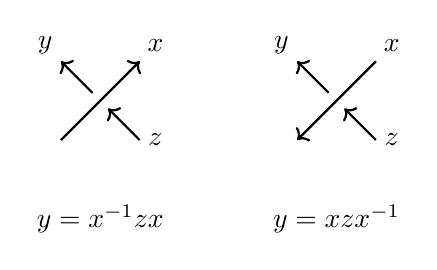
\begin{tikzpicture}
\draw[thick,->] (0,0)--(1,1);
\draw[thick,->] (1,0)--(0.6,0.4);
\draw[thick,->] (0.4,0.6)--(0,1);
\node at (1.2,1.2){$x$};
\node at (-0.2,1.2){$y$};
\node at (1.2,0){$z$};
\node at (0.5,-1){$y=x^{-1}zx$};

\draw[thick,->] (4,1)--(3,0);
\draw[thick,->] (4,0)--(3.6,0.4);
\draw[thick,->] (3.4,0.6)--(3,1);
\node at (4.2,1.2){$x$};
\node at (2.8,1.2){$y$};
\node at (4.2,0){$z$};
\node at (3.5,-1){$y=xzx^{-1}$};

\end{tikzpicture}
    \caption{Types of Crossings}
    \label{fig:wp}
\end{figure}
These generators and relators form a balanced presentation of the fundamental group of the knot complement. Moreover, there exists an ordering of the relators and a choice of $\pm 1$ as exponents such that the relators satisfy the equation
$$\prod_{i=1}^nr_i^{\pm1}=1.
$$
Thus any relator $r_k$ can be eliminated, giving $\langle x_1,\cdots,x_n\mid r_1,\cdots,r_{k-1},r_{k+1},\cdots,r_n\rangle$, without changing the underlying group. When the knot is an unknot, the fundamental group of the knot complement is $\mathbb{Z}$, which can be generated by any generator $x_i$. So after adding a relator $w$ which is any word in $x_1,\ldots,x_n$ with exponent sum $\pm1$, we get a balanced presentation $\langle x_1,\cdots,x_n\mid r_1,\cdots,r_{k-1},r_{k+1},\cdots,r_n,w\rangle$ of the trivial group as in \textbf{Proposition~\ref{prop:unknot}}.

\subsubsection{Reidemeister moves are stable Andrews-Curtis moves} Two diagrams of the same knot can be related by a finite sequence of the three
Reidemeister moves in Figure \ref{fig:rm}. Here we distinguish \textbf{R2a} and \textbf{R2b} just because they give slightly different computation about the presentations. First described in \cite{WADA1994241}, Reidemeister moves can be realized by (AC1)–(AC5). We list the correspondence between Reidemeister moves and (AC1)–(AC5) as follows for self-containment. We consider the presentations obtained from Wirtinger presentations of any unknot diagram by eliminating one arbitrary relator and adding one relator $w$ which is any word in the generators with exponent sum $\pm1$, as described in the previous subsection. Since we want to consider their behavior under Reidemeister moves, we can assume that the relator eliminated is not one given by the crossings in \textbf{R1}, \textbf{R2a}, \textbf{R2b}, \textbf{R3}. We note, however, that since any relator in a Wirtinger presentation can be written as the product of the other relators, the relator we eliminated can be recovered using (AC1)–(AC3).
\\
\\
\textbf{R1}:
\begin{align*}
\langle x_1,\cdots,x_n,x,y\mid r_1,\cdots,r_n,yx^{-1},w\rangle\longleftrightarrow\langle x_1,\cdots,x_n,x\mid r_1',\cdots,r_n',w'\rangle
\end{align*}
Here $r_i'$ and $w'$ are obtained from replacing $y$ in $r_i$ and $w$ by $x$. The equivalence comes from the substitution in \textbf{Lemma~\ref{lem:substitution}}.
\\
\\
\textbf{R2a}:
\begin{align*}
\,\,&\langle x_1,\cdots,x_n,x,y,z,u\mid r_1,\cdots,r_{n+1},xyz^{-1}y^{-1},zy^{-1}u^{-1}y,w\rangle
\\
&\longleftrightarrow\langle x_1,\cdots,x_n,x,y,u\mid r_1',\cdots,r_{n+1}',ux^{-1},w'\rangle
\\
&=\langle x_1,\cdots,x_n,x,y,u\mid r_1,\cdots,r_{n+1},ux^{-1},w'\rangle
\\
&\longleftrightarrow\langle x_1,\cdots,x_n,x,y\mid \tilde{r}_1,\cdots,\tilde{r}_{n+1},\tilde{w}\rangle
\end{align*}
Here $r_i',w'$ are obtained from replacing $z$ in $r_i,w$ by $y^{-1}xy$; $\tilde{r_i}$ from replacing $u$ in $r_i$ by $x$; and $\tilde{w}$ from replacing $u$ in $w'$ by $x$. The second equation comes from the fact that the $r_i$ do not contain $z$.
\\
\textbf{R2b} is similar to \textbf{R2a}.
\\
\\
\textbf{R3}:
\begin{align*}
&\langle x_1,\cdots,x_n,x,y,z,u,v,r\mid r_1,\cdots,r_{n+2},vxy^{-1}x^{-1},urv^{-1}r^{-1},rxz^{-1}x^{-1},w\rangle
\\
&\longleftrightarrow\langle x_1,\cdots,x_n,x,y,z,u,r\mid r_1,\cdots,r_{n+2},urxy^{-1}x^{-1}r^{-1},rxz^{-1}x^{-1},w'\rangle
\\
&\longleftrightarrow\langle x_1,\cdots,x_n,x,y,z,u,r\mid r_1,\cdots,r_{n+2},uxzy^{-1}z^{-1}x^{-1},rxz^{-1}x^{-1},w'\rangle
\\
&\longleftrightarrow\langle x_1,\cdots,x_n,x,y,z,u,r,t\mid r_1,\cdots,r_{n+2},uxzy^{-1}z^{-1}x^{-1},rxz^{-1}x^{-1},tzy^{-1}z^{-1},w'\rangle
\\
&\longleftrightarrow\langle x_1,\cdots,x_n,x,y,z,u,r,t\mid r_1,\cdots,r_{n+2},rxz^{-1}x^{-1},tzy^{-1}z^{-1},uxt^{-1}x^{-1},w'\rangle
\end{align*}
Here $w'$ is obtained from replacing $v$ in $w$ by $xyx^{-1}$.


After reducing our diagram to the trivial diagram of the unknot, we are left with $\langle x \mid \bar w\rangle$, where $\bar w$ is $w$ after applying all the Reidemeister moves. This is because the trivial diagram of the unknot gives the presentation $\langle x\mid \,\,\rangle$ of the infinite cyclic group, so $\bar w$ is the only relator remaining.  Moreover, $\bar w = x^{\pm1}$ since at each stage, $w$ has exponent sum $\pm 1$, so $\langle x \mid \bar w\rangle$ can be reduced to the trivial presentation $\langle \,\, \mid \,\, \rangle$. Thus \textbf{Proposition \ref{prop:unknot}} is proven.

\begin{figure}
    \centering
\begin{tikzpicture}
\draw[thick,rounded corners] (0,0)--(2,0)--(2,-1)--(1,-1)--(1,-0.2);
\draw[thick,rounded corners] (1,0.2)--(1,1);

\draw[<->] (2.5,0)--(3.5,0);

\draw[thick,rounded corners] (4,0)--(5,0)--(5,1);

\node at (4.5,-0.5){$x$};
\node at (0.5,-0.5){$x$};
\node at (1.5,0.5){$y$};

\node at (0.5,0){$>$};
\node at (1,0.5){\rotatebox{90}{$>$}};
\node at (4.5,0){$>$};

\node at (-0.5,0){\textbf{R1}};

\node at (7.5,-3){\textbf{R2b}};

\draw[thick] (9,-2)--(9,-2.3);
\draw[thick] (9,-2.7)--(9,-3.3);
\draw[thick] (9,-3.7)--(9,-4);

\draw[thick,rounded corners] (10,-2)--(10,-2.5)--(8.5,-2.5)--(8.5,-3.5)--(10,-3.5)--(10,-4);

\node at (9,-1.7){$x$};
\node at (10,-1.7){$y$};
\node at (9.2,-3){$z$};
\node at (9,-4.3){$u$};

\node at (9,-2){\rotatebox{90}{$>$}};
\node at (10,-2){\rotatebox{90}{$>$}};
\node at (9,-3){\rotatebox{90}{$>$}};
\node at (9,-3.7){\rotatebox{90}{$>$}};

\draw[<->] (10.5,-3)--(11.5,-3);

\draw[thick] (12.5,-2)--(12.5,-4);
\draw[thick] (13.5,-2)--(13.5,-4);

\node at (12.5,-3){\rotatebox{90}{$>$}};
\node at (13.5,-3){\rotatebox{90}{$>$}};

\node at (12.5,-1.7){$x$};
\node at (13.5,-1.7){$y$};

\draw[thick] (1,-2)--(1,-2.3);
\draw[thick] (1,-2.7)--(1,-3.3);
\draw[thick] (1,-3.7)--(1,-4);

\draw[thick,rounded corners] (2,-2)--(2,-2.5)--(0.5,-2.5)--(0.5,-3.5)--(2,-3.5)--(2,-4);

\node at (1,-2){\rotatebox{90}{$>$}};
\node at (2,-2.3){\rotatebox{90}{$<$}};
\node at (1,-3){\rotatebox{90}{$>$}};
\node at (1,-3.7){\rotatebox{90}{$>$}};

\draw[<->] (2.5,-3)--(3.5,-3);

\draw[thick] (4.5,-2)--(4.5,-4);
\draw[thick] (5.5,-2)--(5.5,-4);

\node at (4.5,-3){\rotatebox{90}{$>$}};
\node at (5.5,-3){\rotatebox{90}{$<$}};

\node at (4.5,-1.7){$x$};
\node at (5.5,-1.7){$y$};

\node at (1,-1.7){$x$};
\node at (2,-1.7){$y$};
\node at (1.2,-3){$z$};
\node at (1,-4.3){$u$};

\node at (-0.5,-3){\textbf{R2a}};

\draw[thick] (1,-5)--(1,-8);
\draw[thick] (0.5,-7.5)--(0.8,-7.5);
\draw[thick,rounded corners] (1.2,-7.5)--(2,-7.5)--(2,-5.5)--(3.5,-5.5);
\draw[thick] (0.5,-6.5)--(0.8,-6.5);
\draw[thick] (1.2,-6.5)--(1.8,-6.5);
\draw[thick] (2.2,-6.5)--(3.5,-6.5);

\draw[<->] (4,-6.5)--(5,-6.5);

\draw[thick] (5.5,-6.5)--(6.8,-6.5);
\draw[thick,rounded corners] (5.5,-7.5)--(7,-7.5)--(7,-5.5)--(7.8,-5.5);
\draw[thick,rounded corners] (7.2,-6.5)--(7.8,-6.5);
\draw[thick] (8,-5)--(8,-8);
\draw[thick] (8.2,-5.5)--(8.5,-5.5);
\draw[thick] (8.2,-6.5)--(8.5,-6.5);

\node at (0.5,-5.5){$x$};
\node at (0.5,-6.2){$y$};
\node at (0.5,-7.2){$z$};
\node at (3,-5.2){$r$};
\node at (3,-6.2){$u$};
\node at (1.5,-6.2){$v$};

\node at (1,-5.5){\rotatebox{90}{$>$}};
\node at (0.7,-6.5){$>$};
\node at (0.7,-7.5){$>$};
\node at (1.5,-6.5){$>$};
\node at (3,-5.5){$>$};
\node at (3,-6.5){$>$};

\node at (8,-4.5){$x$};
\node at (6,-6.2){$y$};
\node at (6,-7.2){$z$};
\node at (9,-5.5){$r$};
\node at (9,-6.5){$u$};
\node at (7.5,-6.2){$t$};

\node at (8,-5){\rotatebox{90}{$>$}};
\node at (6,-6.5){$>$};
\node at (6,-7.5){$>$};
\node at (8.5,-6.5){$>$};
\node at (8.5,-5.5){$>$};
\node at (7.5,-6.5){$>$};

\node at (-0.5,-6){\textbf{R3}};

\end{tikzpicture}
    \caption{Reidemeister moves}
    \label{fig:rm}
\end{figure}


\subsubsection{Constructing Infinite Familes}
Any diagram of the unknot with $n$ crossings gives us $n$ examples of infinite families of presentations that are known to be stably AC-trivial, as given by the proposition.

Moreover, we can use stable AC-moves, especially the substitution move in Lemma~\ref{lem:substitution}, to reduce the number of generators and relations in these families of presentations. Indeed, if we restrict our attention to the relators coming from the Wirtinger presentation (i.e., without changing the free choice of $w$), we can get similar infinite families of presentations with fewer generators. This is valuable since most of the focus in studying the (stable) Andrews-Curtis conjecture is given to presentations with a small number of generators, especially 2 and 3.

\begin{remark}
This approach can at best generate interesting infinite families with three generators and relators, since removing $w$ will always give us a presentation of $\mathbb{Z}$ and so any two-generator presentation must be just $\langle x,y \mid x=\pm y, w\rangle$.
\end{remark}
\begin{remark}
    Each infinite family coming from Proposition~\ref{prop:unknot} will give many distinct infinite families with fewer generators, as we have many different ways to simplify the groups that lead to different presentations.
\end{remark}
\begin{remark}
    In order to get interesting examples, it seems sensible to look at hard unknot diagrams, as the easier it is to change the diagram into the trivial diagram of the unknot, the easier it should be for the computer algorithms to trivialize the resulting presentations.
\end{remark}
\begin{remark}
    On the other hand, the more complicated the knot diagram, the harder it will be to simplify the presentation down to three generators, and the less likely such a presentation is of reasonable length.
\end{remark}
\begin{remark}
    We can also make presentations more complicated by choosing simplification steps that make the presentation more complicated. However it seems more likely to get interesting presentations from choosing a complicated knot diagram and simplifying more.
\end{remark}

\begin{conjecture}
    Every stably AC-trivial presentation of the form from Proposition~\ref{prop:unknot} can also be stably AC-trivialized without (AC4), and in particular by just doing substitutions.
\end{conjecture}

Note that realizing Reidemeister moves with stable AC moves \emph{does} require (AC4), and thus this conjecture is not a consequence of the proof of the proposition. We checked that it holds in many of hard unknot diagrams in \cite{burton2021harddiagramsunknot}, in particular for the Culprit, D28, Goeritz, Ochai I, and Tuzun Sikora.

If true, it provides some evidence against this approach generating lots of interesting examples of stably AC-trivial presentations.
\subsubsection{Examples}
One famous hard unknot diagram is the 10-crossing Culprit, first introduced in \cite{kauffman2014hardunknotscollapsingtangles}. One possibly interesting infinite family coming from this diagram is the following:
\begin{proposition}
    Any presentation of the form
    \[
\langle x,y,z \,\mid \, xzxz^{-1}x^{-1}yzyz^{-1}y^{-1}z^{-1}y^{-1}, zx^{-1}yzy^{-1}z^{-1}y^{-1}x, w \rangle,
\] where $w$ is a word with exponent sum $\pm 1$, is a stably AC-trivial presentation of the trivial group. [is it worth showing the substitution steps of how you get this presentation from the culprit?]
\end{proposition}
However, it is difficult to find a choice of $w$ that gives any non-trivial result. For example, if $w=z^{-1}w'$, where $w'$ is a word in $x$ and $y$ of length $\leq 8$, then the greedy search is able to instantly trivialize the presentation.
	\appendix
	% !TEX root = ../ac_paper.tex

\section{Hyperparameters\label{app:hyperparameters}}

Here we discuss the hyperparameters we used to train our Proximal Policy Optimization and Transformer models discussed in the main text. 

\fixme{Insert details of PPO hyperparameters here.}

We used an 8-layer transformer model with the embedding space dimension of $512$ and 4 attention heads. The context window of the Transformer had length 1024. We used a batch size of $12$ and constant learning rate of $6 \times 10^{-5}$. We trained for a total of 25000 iterations. We used Adam hyperparameters $\beta_1 = 0.9$, $\beta_2 = 0.99$ and a dropout value of $0$.
   	 \input{app/ac_paths}
        %% !TEX root = ../ac_paper.tex

\section{RL path \label{app:RLpath}}

\[
\begin{aligned}
& h_{2} \cdot h_{8} \cdot h_{6} \cdot h_{4} \cdot h_{10} \cdot h_{2} \cdot h_{8} \cdot h_{6} \cdot h_{6} \cdot h_{8} \cdot h_{10} \cdot h_{10} \cdot h_{10} \cdot h_{7} \cdot h_{0} \cdot h_{4} \cdot h_{6} \cdot h_{6} \\ &
h_{6} \cdot h_{6} \cdot h_{11} \cdot h_{8} \cdot h_{10} \cdot h_{10} \cdot h_{2} \cdot h_{8} \cdot h_{6} \cdot h_{4} \cdot h_{10} \cdot h_{2} \cdot h_{8} \cdot h_{6} \cdot h_{6} \cdot h_{6} \cdot h_{8} \cdot h_{10} \\ &
h_{10} \cdot h_{10} \cdot h_{7} \cdot h_{3} \cdot h_{5} \cdot h_{5} \cdot h_{5} \cdot h_{0} \cdot h_{4} \cdot h_{6} \cdot h_{11} \cdot h_{5} \cdot h_{9} \cdot h_{7} \cdot h_{11} \cdot h_{7} \cdot h_{11} \cdot h_{5} \\ &
h_{4} \cdot h_{9} \cdot h_{2} \cdot h_{8} \cdot h_{6} \cdot h_{6} \cdot h_{6} \cdot h_{8} \cdot h_{10} \cdot h_{8} \cdot h_{10} \cdot h_{10} \cdot h_{4} \cdot h_{7} \cdot h_{0} \cdot h_{4} \cdot h_{6} \cdot h_{11} \\ &
h_{2} \cdot h_{8} \cdot h_{6} \cdot h_{6} \cdot h_{8} \cdot h_{10} \cdot h_{8} \cdot h_{10} \cdot h_{2} \cdot h_{8} \cdot h_{4} \cdot h_{10} \cdot h_{7} \cdot h_{0} \cdot h_{4} \cdot h_{6} \cdot h_{4} \cdot h_{11} \\ &
h_{10} \cdot h_{2} \cdot h_{8} \cdot h_{6} \cdot h_{4} \cdot h_{10} \cdot h_{8} \cdot h_{7} \cdot h_{0} \cdot h_{4} \cdot h_{6} \cdot h_{11} \cdot h_{4} \cdot h_{7} \cdot h_{11} \cdot h_{2} \cdot h_{8} \cdot h_{6} \\ &
h_{2} \cdot h_{8} \cdot h_{6} \cdot h_{8} \cdot h_{8} \cdot h_{10} \cdot h_{7} \cdot h_{0} \cdot h_{4} \cdot h_{0} \cdot h_{4} \cdot h_{0} \cdot h_{4} \cdot h_{0} \cdot h_{4} \cdot h_{6} \cdot h_{11} \cdot h_{2} \\ &
h_{8} \cdot h_{6} \cdot h_{4} \cdot h_{6} \cdot h_{8} \cdot h_{8} \cdot h_{10} \cdot h_{10} \cdot h_{10} \cdot h_{10} \cdot h_{2} \cdot h_{8} \cdot h_{6} \cdot h_{4} \cdot h_{10} \cdot h_{8} \cdot h_{7} \cdot h_{0} \\ &
h_{4} \cdot h_{6} \cdot h_{11} \cdot h_{4} \cdot h_{2} \cdot h_{8} \cdot h_{6} \cdot h_{6} \cdot h_{8} \cdot h_{8} \cdot h_{10} \cdot h_{10} \cdot h_{7} \cdot h_{0} \cdot h_{4} \cdot h_{0} \cdot h_{4} \cdot h_{6} \\ &
h_{11} \cdot h_{8} \cdot h_{7} \cdot h_{11} \cdot h_{5} \cdot h_{4} \cdot h_{8} \cdot h_{11} \cdot h_{7} \cdot h_{4} \cdot h_{8} \cdot h_{11} \cdot h_{7} \cdot h_{9} \cdot h_{6} \cdot h_{8} \cdot h_{8} \cdot h_{10} \\ &
h_{4} \cdot h_{10} \cdot h_{10} \cdot h_{8} \cdot h_{2} \cdot h_{8} \cdot h_{6} \cdot h_{7} \cdot h_{8} \cdot h_{11} \cdot h_{8} \cdot h_{10} \cdot h_{4} \cdot h_{10} \cdot h_{10} \cdot h_{2} \cdot h_{8} \cdot h_{6} \\ &
h_{4} \cdot h_{6} \cdot h_{8} \cdot h_{8} \cdot h_{8} \cdot h_{10} \cdot h_{7} \cdot h_{11} \cdot h_{7} \cdot h_{4} \cdot h_{11} \cdot h_{10} \cdot h_{7} \cdot h_{0} \cdot h_{4} \cdot h_{6} \cdot h_{11} \cdot h_{4} \\ &
h_{2} \cdot h_{8} \cdot h_{6} \cdot h_{8} \cdot h_{8} \cdot h_{8} \cdot h_{10} \cdot h_{7} \cdot h_{0} \cdot h_{4} \cdot h_{0} \cdot h_{4} \cdot h_{0} \cdot h_{4} \cdot h_{6} \cdot h_{8} \cdot h_{11} \cdot h_{2} \\ &
h_{8} \cdot h_{8} \cdot h_{10} \cdot h_{10} \cdot h_{10} \cdot h_{2} \cdot h_{8} \cdot h_{2} \cdot h_{8} \cdot h_{6} \cdot h_{4} \cdot h_{6} \cdot h_{8} \cdot h_{10} \cdot h_{8} \cdot h_{10} \cdot h_{10} \cdot h_{7} \\ &
h_{0} \cdot h_{4} \cdot h_{6} \cdot h_{11} \cdot h_{4} \cdot h_{2} \cdot h_{8} \cdot h_{6} \cdot h_{4} \cdot h_{2} \cdot h_{8} \cdot h_{6} \cdot h_{8} \cdot h_{10} \cdot h_{7} \cdot h_{11} \cdot h_{7} \cdot h_{5} \\ &
h_{11} \cdot h_{8} \cdot h_{10} \cdot h_{4} \cdot h_{8} \cdot h_{9} \cdot h_{7} \cdot h_{4} \cdot h_{8} \cdot h_{9} \cdot h_{7} \cdot h_{0} \cdot h_{4} \cdot h_{0} \cdot h_{4} \cdot h_{6} \cdot h_{11} \cdot h_{5} \\ &
h_{9} \cdot h_{4} \cdot h_{2} \cdot h_{8} \cdot h_{6} \cdot h_{4} \cdot h_{6} \cdot h_{8} \cdot h_{8} \cdot h_{10} \cdot h_{10} \cdot h_{7} \cdot h_{0} \cdot h_{4} \cdot h_{6} \cdot h_{11} \cdot h_{6} \cdot h_{8} \\ &
h_{8} \cdot h_{10} \cdot h_{4} \cdot h_{10} \cdot h_{2} \cdot h_{8} \cdot h_{6} \cdot h_{8} \cdot h_{8} \cdot h_{10} \cdot h_{7} \cdot h_{11} \cdot h_{7} \cdot h_{5} \cdot h_{11} \cdot h_{9} \cdot h_{7} \cdot h_{9} \\ &
h_{7} \cdot h_{4} \cdot h_{0} \cdot h_{4} \cdot h_{6} \cdot h_{11} \cdot h_{8} \cdot h_{8} \cdot h_{8} \cdot h_{10} \cdot h_{7} \cdot h_{0} \cdot h_{4} \cdot h_{6} \cdot h_{4} \cdot h_{11} \cdot h_{10} \cdot h_{2} \\ &
h_{8} \cdot h_{8} \cdot h_{8} \cdot h_{10} \cdot h_{7} \cdot h_{0} \cdot h_{4} \cdot h_{6} \cdot h_{11} \cdot h_{4} \cdot h_{2} \cdot h_{8} \cdot h_{8} \cdot h_{2} \cdot h_{8} \cdot h_{10} \cdot h_{2} \cdot h_{8} \\ &
h_{6} \cdot h_{4} \cdot h_{6} \cdot h_{8} \cdot h_{10} \cdot h_{7} \cdot h_{0} \cdot h_{4} \cdot h_{6} \cdot h_{11} \cdot h_{8} \cdot h_{8} \cdot h_{8} \cdot h_{8} \cdot h_{8} \cdot h_{8} \cdot h_{8} \cdot h_{1} \\ &
h_{7} \cdot h_{5} \cdot h_{11}
\end{aligned}
\]
	% !TEX root = ../ac_paper.tex

\section{Neighborhood constructions}\label{s:neighborhoods}

\subsection{Neighborhoods of the identity}

For any $\ell \in \{3, \dots, 16\}$, we constructed a neighborhood of the identity using an algorithm based on BFS search (\autoref{alg:bfs_1}).
This neighborhood contains all presentations that can be connected to the identity via a path of AC moves, where each presentation in the path has a length less than or equal to $\ell$, that is, the full based subgraph containing vertices with connectivity value less than or equal to $\ell$.
We consider the relators of a presentations as a set (meaning that the order of relators is not important; implemented as a tuple of relators in lexicographic order) 

\begin{algorithm}
	\caption{Breadth-First Search Algorithm Bounded by Size}
    \label{alg:bfs_1}
	\begin{algorithmic}[1]
		\State \textbf{Input:} A balanced presentation $\pi$, maximal size of presentation $n$
		\State \textbf{Output:} Set of enumerated presentations connected to the starting presentation that are achievable without exceeding the size limit, and set of edges with filtrations
		\State Initialize a queue $Q$, set of visited nodes $visited$, and numerical map $name$ that will enumerate presentations
		\State Mark $\pi$ as visited, put it into queue $Q$, and assign it the number $0$
		\While{$Q$ is not empty}
		\State $u \gets $ top of $Q$ \Comment{Remove the front node of $Q$}
		\For{every AC move $m$}
		\State $child \gets m(u)$
		\If{$child$'s size $\leq n$ and $child$ is not visited}
		\State Put $child$ in $Q$ and mark it as visited
		\State Assign $child$ the next available number
		\EndIf
		\If{$child$'s size $\leq n$ and $u$'s number is smaller than $child$'s number}
		\State Return edge $(u, child)$ with proper filtration
		\EndIf
		\EndFor
		\EndWhile
	\end{algorithmic}
\end{algorithm}

\subsection{Neighborhoods for MS series}

We define the $n$-neighborhood of a balanced presentation $\pi$ as the set of all balanced presentations that can be obtained by applying at most $n$ AC-moves to $\pi$.
We used \autoref{alg:bfs_neigh}, a variation of BFS, to generate $5$-neighborhoods of presentations in the Miller--Schupp series. 
As before, we disregard the order of the relators.

\begin{algorithm}
	\caption{Breadth-First Search Algorithm Bounded by Number of Steps}\label{alg:bfs_neigh}
	\begin{algorithmic}[1]
		\State \textbf{Input:} A balanced presentation $\pi$, positive integer $n$
		\State \textbf{Output:} $n$-neighborhood of $\pi$
		\State Initialize a queue $Q$, set of visited nodes $visited$, and numerical map $dist$ that represents the minimal number of AC-moves needed to transform $\pi$ into a given presentation
		\State Mark $\pi$ as visited, put it into queue $Q$, and set its distance to $0$
		\While{$Q$ is not empty}
		\State $u \gets $ top of $Q$ \Comment{Remove the front node of $Q$}
		\For{every AC move $m$}
		\State $child \gets m(u)$
		\If{$dist[u] < n$ and $child$ is not in $visited$}
		\State Put $child$ in $Q$ and mark it as visited
		\State Set $dist[child] := dist[u] + 1$
		\EndIf
		\EndFor
		\EndWhile
		\Return set $visited$
	\end{algorithmic}
\end{algorithm}
	% !TEX root = ../ac_paper.tex

\section{Language Modeling Dataset Generation \label{app:algorithm}}

This appendix describes the method, \autoref{alg:apply_ac_moves}, used to generate the training and evaluation datasets for the Transformer model, as referenced in \autoref{sec:lm}. Our aim was to create datasets featuring presentations of varying lengths. We began with a presentation \(P_0\) from the Miller--Schupp series, where \(n, \length(w) \leq 7\), setting a maximum relator length \(l_{\text{max}} = 128\). Presentations were generated in \(n=128\) phases, each phase allowing a maximum relator length \(l_i \sim \mathcal{U}(l + i \cdot l_{\text{inc}}, l + (i+1) \cdot l_{\text{inc}})\). Here, \(l\) represents the longest relator length in \(P_0\) and \(l_{\text{inc}} = (l_{\text{max}} - l)/n\) is the incremental increase per phase. In each phase, we selected a presentation \(P\) from the previous phase and applied \(N=1000\) AC$'$ moves. Any AC$'$ move that exceeded the length \(l_i\) resulted in no change.


We repeated this for all 1190 presentations in the Miller--Schupp series, ultimately producing approximately 1.8 million balanced presentations. The length distribution of these presentations is detailed in \autoref{fig:gpt_data}.

\begin{algorithm}
    \caption{Transformer Dataset Generation}
    \label{alg:apply_ac_moves}
    \begin{algorithmic}[1]
        \State \textbf{Input:}
     	\begin{itemize}
	\item[]     $P_0$  --- an initial presentation with $l$ as the length of the longest relator
          \item[]   $n$  --- number of phases
           \item[]  $m$  --- number of presentations in each phase
           \item[]  $N$  --- number of AC$'$ moves to apply in each phase
         \item[]    $l_{\text{max}}$  --- upper bound on presentation lengths in the dataset
          \end{itemize}
         \State \textbf{Output:}
         \begin{itemize}
         \item[]         Dataset (the final collection of presentations)
         \end{itemize}
        \State Dataset $\gets \emptyset$ \Comment{Initialize the dataset of all presentations}
        \State $l_{\text{inc}} \gets (l_{\text{max}} - l) / n$ \Comment{Increment for the maximum relator length per phase}
        \For{$i = 0$ \textbf{to} $n-1$} \Comment{Loop over each phase}
            \For{$j = 1$ \textbf{to} $m$} \Comment{Generate $m$ presentations for each phase}
                \State $l_i \sim \mathcal{U}(l + i \cdot l_{\text{inc}}, l + (i+1) \cdot l_{\text{inc}})$
                \Comment{Sample maximum relator length}
		\State $P \gets (i = 1) \ ? \ P_0 \ : \ \text{Dataset}[(i-1) \cdot m + j - 1]$
                \For{$k = 1$ \textbf{to} $N$} \Comment{Apply $N$ AC$'$ moves with relator length $l_i$}
                    \State $A \sim \text{AC}' \text{ Moves}$
                    \State $P \gets A \cdot P$
                \EndFor
                \State Dataset $\gets$ Dataset $\cup \{P\}$
                \Comment{Add the presentation $P$ to the Dataset}
            \EndFor
        \EndFor
    \end{algorithmic}
\end{algorithm}




    \section{Reidemeister moves realized by stable AC moves}\label{app:reid}

In this appendix, we prove \cref{prop:unknot-stable}, which we rewrite below.

\begin{proposition}[Myasnikov, Myasnikov, and Shpilrain, \cite{MMS}]
    Let $\angles{ x_1,\ldots, x_n\, \mid \, r_1, \ldots, r_n }$ be the Wirtinger presentation of an unknot diagram. Then for any $k=1,\ldots,n$ and word $w$ in the $x_i$ with exponent sum $\pm 1$, the balanced presentation of the trivial group $\langle x_1,\ldots, x_n\,|\, r_1,\ldots, r_{k-1}, r_{k+1},\ldots, r_n, w\rangle$ is stably Andrews-Curtis-trivial.
\end{proposition}

As reviewed in \cref{subsec:ac-unknot}, given any oriented knot diagram, we assign generators $\{x_i\}_{i=1}^n$ to each of the arcs and relators $\{ r_i\}_{i=1}^n$ to each of the crossings. These generators and relators form a balanced presentation of the fundamental group of the knot complement. There exists an ordering of the relators and a choice of $\pm 1$ as exponents such that the relators satisfy the equation, 
\[
\prod\limits_{i=1}^n r_i^{\pm 1} = 1
\]
Thus any relator can be eliminated, giving $\angles{x_1, \dots , x_n \mid r_1, \dots, r_{k-1}, r_{k+1}, \dots, r_n }$ without changing the underlying group. When the knot is an unknot, adding a relator $w$, which is a word in $x_1, \dots , x_n$ with exponent sum $\pm 1$, gives a balanced presentation of the trivial group $\angles{x_1, \dots , x_n \mid r_1, \dots, r_{k-1}, r_{k+1}, \dots, r_n , w}$. 

Here, we will show that the application of Reidemeister moves to a knot diagram of the unknot corresponds to application of stable AC moves (AC1)--(AC5) to the associated balanced presentation of the trivial group. This relationship was first studied in \cite{WADA1994241}.
%\footnote{A similar relationship between Reidemeister moves applied to a knot diagram and the application of stable AC moves to the associated Wirtinger presentation was given in \cite{WADA1994241}. }
%The proof presented here as the advantage that the effect of stable AC moves on $w$ is explicit.
%\shehper{@Lucas: can you please independently check that \cite{WADA1994241} discuss the effect of stable AC moves on Wirtinger presentation and not on the balanced presentation, And hence, they do not show how these moves effect $w$? If not, we can remove the second sentence of the footnote.}
%\lucas{@Shehper: I agree they do not explicitly show it in Wada, although the effect on $w$ part is pretty trivial}}
%\shehper{@Lucas: okay, thank you. I have edited the footnote.}
As a knot diagram of the unknot is reduced to the trivial diagram, the associated balanced presentation is shown to be stably AC-trivial.

\begin{figure}
    \centering
\begin{tikzpicture}
\draw[thick,rounded corners] (0,0)--(2,0)--(2,-1)--(1,-1)--(1,-0.2);
\draw[thick,rounded corners] (1,0.2)--(1,1);

\draw[<->] (2.5,0)--(3.5,0);

\draw[thick,rounded corners] (4,0)--(5,0)--(5,1);

\node at (4.5,-0.5){$x$};
\node at (0.5,-0.5){$x$};
\node at (1.5,0.5){$y$};

\node at (0.5,0){$>$};
\node at (1,0.5){\rotatebox{90}{$>$}};
\node at (4.5,0){$>$};

\node at (-0.5,0){\textbf{R1}};

\node at (7.5,-3){\textbf{R2b}};

\draw[thick] (9,-2)--(9,-2.3);
\draw[thick] (9,-2.7)--(9,-3.3);
\draw[thick] (9,-3.7)--(9,-4);

\draw[thick,rounded corners] (10,-2)--(10,-2.5)--(8.5,-2.5)--(8.5,-3.5)--(10,-3.5)--(10,-4);

\node at (9,-1.7){$x$};
\node at (10,-1.7){$y$};
\node at (9.2,-3){$z$};
\node at (9,-4.3){$u$};

\node at (9,-2){\rotatebox{90}{$>$}};
\node at (10,-2){\rotatebox{90}{$>$}};
\node at (9,-3){\rotatebox{90}{$>$}};
\node at (9,-3.7){\rotatebox{90}{$>$}};

\draw[<->] (10.5,-3)--(11.5,-3);

\draw[thick] (12.5,-2)--(12.5,-4);
\draw[thick] (13.5,-2)--(13.5,-4);

\node at (12.5,-3){\rotatebox{90}{$>$}};
\node at (13.5,-3){\rotatebox{90}{$>$}};

\node at (12.5,-1.7){$x$};
\node at (13.5,-1.7){$y$};

\draw[thick] (1,-2)--(1,-2.3);
\draw[thick] (1,-2.7)--(1,-3.3);
\draw[thick] (1,-3.7)--(1,-4);

\draw[thick,rounded corners] (2,-2)--(2,-2.5)--(0.5,-2.5)--(0.5,-3.5)--(2,-3.5)--(2,-4);

\node at (1,-2){\rotatebox{90}{$>$}};
\node at (2,-2.3){\rotatebox{90}{$<$}};
\node at (1,-3){\rotatebox{90}{$>$}};
\node at (1,-3.7){\rotatebox{90}{$>$}};

\draw[<->] (2.5,-3)--(3.5,-3);

\draw[thick] (4.5,-2)--(4.5,-4);
\draw[thick] (5.5,-2)--(5.5,-4);

\node at (4.5,-3){\rotatebox{90}{$>$}};
\node at (5.5,-3){\rotatebox{90}{$<$}};

\node at (4.5,-1.7){$x$};
\node at (5.5,-1.7){$y$};

\node at (1,-1.7){$x$};
\node at (2,-1.7){$y$};
\node at (1.2,-3){$z$};
\node at (1,-4.3){$u$};

\node at (-0.5,-3){\textbf{R2a}};

\draw[thick] (1,-5)--(1,-8);
\draw[thick] (0.5,-7.5)--(0.8,-7.5);
\draw[thick,rounded corners] (1.2,-7.5)--(2,-7.5)--(2,-5.5)--(3.5,-5.5);
\draw[thick] (0.5,-6.5)--(0.8,-6.5);
\draw[thick] (1.2,-6.5)--(1.8,-6.5);
\draw[thick] (2.2,-6.5)--(3.5,-6.5);

\draw[<->] (4,-6.5)--(5,-6.5);

\draw[thick] (5.5,-6.5)--(6.8,-6.5);
\draw[thick,rounded corners] (5.5,-7.5)--(7,-7.5)--(7,-5.5)--(7.8,-5.5);
\draw[thick,rounded corners] (7.2,-6.5)--(7.8,-6.5);
\draw[thick] (8,-5)--(8,-8);
\draw[thick] (8.2,-5.5)--(8.5,-5.5);
\draw[thick] (8.2,-6.5)--(8.5,-6.5);

\node at (0.5,-5.5){$x$};
\node at (0.5,-6.2){$y$};
\node at (0.5,-7.2){$z$};
\node at (3,-5.2){$r$};
\node at (3,-6.2){$u$};
\node at (1.5,-6.2){$v$};

\node at (1,-5.5){\rotatebox{90}{$>$}};
\node at (0.7,-6.5){$>$};
\node at (0.7,-7.5){$>$};
\node at (1.5,-6.5){$>$};
\node at (3,-5.5){$>$};
\node at (3,-6.5){$>$};

\node at (8,-4.5){$x$};
\node at (6,-6.2){$y$};
\node at (6,-7.2){$z$};
\node at (9,-5.5){$r$};
\node at (9,-6.5){$u$};
\node at (7.5,-6.2){$t$};

\node at (8,-5){\rotatebox{90}{$>$}};
\node at (6,-6.5){$>$};
\node at (6,-7.5){$>$};
\node at (8.5,-6.5){$>$};
\node at (8.5,-5.5){$>$};
\node at (7.5,-6.5){$>$};

\node at (-0.5,-6){\textbf{R3}};

\end{tikzpicture}
    \caption{Reidemeister moves}
    \label{fig:rm}
\end{figure}

Two diagrams of the same knot can be related by a finite sequence of the three
Reidemeister moves shown in \cref{fig:rm}. Here we distinguish \textbf{R2a} and \textbf{R2b} just because they give slightly different computation about the presentations. Since we want to consider the behavior of balanced presentations $\angles{ x_1,\ldots, x_n \mid  r_1,\ldots, r_{k-1}, r_{k+1},\ldots, r_n, w}$ of the trivial group under Reidemeister moves, we can assume that the relator eliminated, $r_k$, is not one given by the crossings in \textbf{R1}, \textbf{R2a}, \textbf{R2b}, \textbf{R3}. We note, however, that since any relator in a Wirtinger presentation can be written as the product of the other relators, the relator we eliminated can be recovered using (AC1)--(AC3).
\\
\\
\textbf{R1}:
\begin{align*}
\langle x_1,\ldots,x_n,x,y\mid r_1,\ldots,r_n,yx^{-1},w\rangle\longleftrightarrow\langle x_1,\ldots,x_n,x\mid r_1',\ldots,r_n',w'\rangle
\end{align*}
Here $r_i'$ and $w'$ are obtained from replacing $y$ in $r_i$ and $w$ by $x$. The equivalence comes from the substitution in \cref{lem:substitution}.
\\
\\
\textbf{R2a}:
\begin{align*}
\,\,&\langle x_1,\ldots,x_n,x,y,z,u\mid r_1,\ldots,r_{n+1},xyz^{-1}y^{-1},zy^{-1}u^{-1}y,w\rangle
\\
&\longleftrightarrow\langle x_1,\ldots,x_n,x,y,u\mid r_1',\ldots,r_{n+1}',ux^{-1},w'\rangle
\\
&=\langle x_1,\ldots,x_n,x,y,u\mid r_1,\ldots,r_{n+1},ux^{-1},w'\rangle
\\
&\longleftrightarrow\langle x_1,\ldots,x_n,x,y\mid \tilde{r}_1,\ldots,\tilde{r}_{n+1},\tilde{w}\rangle
\end{align*}
Here $r_i',w'$ are obtained from replacing $z$ in $r_i,w$ by $y^{-1}xy$; $\tilde{r_i}$ from replacing $u$ in $r_i$ by $x$; and $\tilde{w}$ from replacing $u$ in $w'$ by $x$. The second equation comes from the fact that the $r_i$ do not contain $z$.
\\
\textbf{R2b} is similar to \textbf{R2a}.
\\
\\
\textbf{R3}:
\begin{align*}
&\langle x_1,\ldots,x_n,x,y,z,u,v,r\mid r_1,\ldots,r_{n+2},vxy^{-1}x^{-1},urv^{-1}r^{-1},rxz^{-1}x^{-1},w\rangle
\\
&\longleftrightarrow\langle x_1,\ldots,x_n,x,y,z,u,r\mid r_1,\ldots,r_{n+2},urxy^{-1}x^{-1}r^{-1},rxz^{-1}x^{-1},w'\rangle
\\
&\longleftrightarrow\langle x_1,\ldots,x_n,x,y,z,u,r\mid r_1,\ldots,r_{n+2},uxzy^{-1}z^{-1}x^{-1},rxz^{-1}x^{-1},w'\rangle
\\
&\longleftrightarrow\langle x_1,\ldots,x_n,x,y,z,u,r,t\mid r_1,\ldots,r_{n+2},uxzy^{-1}z^{-1}x^{-1},rxz^{-1}x^{-1},tzy^{-1}z^{-1},w'\rangle
\\
&\longleftrightarrow\langle x_1,\ldots,x_n,x,y,z,u,r,t\mid r_1,\ldots,r_{n+2},rxz^{-1}x^{-1},tzy^{-1}z^{-1},uxt^{-1}x^{-1},w'\rangle
\end{align*}
Here $w'$ is obtained from replacing $v$ in $w$ by $xyx^{-1}$.


After reducing our diagram to the trivial diagram of the unknot, we are left with $\langle x \mid \bar w\rangle$, where $\bar w$ is $w$ after applying all the Reidemeister moves. This is because the trivial diagram of the unknot gives the presentation $\langle x\mid \,\,\rangle$ of the infinite cyclic group, so $\bar w$ is the only relator remaining.  Moreover, $\bar w = x^{\pm1}$ since at each stage, $w$ has exponent sum $\pm 1$, so $\langle x \mid \bar w\rangle$ can be reduced to the trivial presentation $\langle \,\, \mid \,\, \rangle$. Thus \cref{prop:unknot-stable} is proven.


    % !TEX root = ../ac_paper.tex

\section{A misprint in the Wirtinger presentation of \cite{MMS}.}  \label{app:mms}
The unknot diagram of \cref{fig:unknot} was originally presented in \cite{MMS}. Their manuscript contained an unfortunate misprint in the 13th relator, where it is written as $x_{13}=x_5 x_{12} x_5^{-1}$.  The resultant presentation—denoted $W’$—is not a Wirtinger presentation of any knot diagram. In a Wirtinger presentation, any single relator is redundant, meaning that removing any relator still yields a valid presentation of the knot group. In the case of an unknot, this group is the infinite cyclic group $\mathbb{Z}$. However, removing different relators from $W’$ produces different groups. For instance, if the relator $x_{7} = x_4^{-1} x_{6} x_4$ is removed, the resulting group is the three-strand braid group, whereas removing $x_{14} = x_1 x_{13} x_1^{-1}$ yields $\mathbb{Z}$.

In \cite[Theorem 1.4]{MMS}, the following 3-generator family of presentations,
\[
\angles{ x,y,z \mid  x=z\cdot [[y^{-1},x^{-1}],z], y=x\cdot [[y^{-1},x^{-1}],z^{-1}]\cdot [z^{-1},x], w},
\] 
was obtained by deleting the 12th relator from $W'$, adding $w$, and then recursively eliminating other generators. The theorem statement claimed that every element of this 3-generator family presents the trivial group. However, due to the misprint, $W'$ with the 12th relator eliminated is not a presentation of $\mathbb{Z}$.

Despite this error, it is possible to get presentations of the trivial group after choosing appropriate $w$. For example, when $w = x^{-1} y z$, the 3-generator presentation is stably AC-equivalent to a length $25$ presentation,
\[
\langle x, y \mid
	x^{-1}y^{-1}xy^{-1}x^{-1}yxy^{-2}xyx^{-1}y, \
	y^{-1}x^{-1}y^2x^{-1}y^{-1}xyxy^{-2}x 
\rangle,
\]
which is AC-equivalent to $\AK(3)$. Note, however, that unlike any presentation AC-equivalent to a correct Wirtinger presentation, these presentations are not necessarily stably AC-trivial. For completeness, we provide the AC path that connects the length $25$ presentation to $\AK(3)$,
\[
\begin{aligned}
& h_9 \cdot h_7 \cdot h_4 \cdot h_8 \cdot h_{11} \cdot h_5 \cdot h_{11} \cdot h_9 \cdot h_3 \cdot h_{10} \cdot h_{12} \cdot h_7 \cdot h_7 \cdot h_9 \cdot h_{11} \cdot h_5 \cdot h_3 \cdot h_5 \cdot \\
& h_4 \cdot h_3 \cdot h_{12} \cdot h_5 \cdot h_7 \cdot h_7 \cdot h_1 \cdot h_9 \cdot h_{11} \cdot h_8 \cdot h_3 \cdot h_5 \cdot h_{10} \cdot h_2 \cdot h_6 \cdot h_{12} \cdot h_9 \cdot h_7 \cdot \\
& h_5 \cdot h_{11} \cdot h_{10} \cdot h_3 \cdot h_8 \cdot h_{11} \cdot h_9 \cdot h_2 \cdot h_{10} \cdot h_{12} \cdot h_5 \cdot h_7 \cdot h_9 \cdot h_{11} \cdot h_1 \cdot h_9 \cdot h_8.
\end{aligned}
\]
Here, $h_i$ are AC$'$ moves as defined in \cref{app:paths}. 



        %\input{app/families}
        %% !TEX root = ../ac_paper.tex

\subsection{Proof of Theorem \ref{thm:stableAK3}}
%\section{Stable AC-trivialization of $\AK(3)$}
\label{sec:stable_ak3}
\anibal{To decide what to do with this subsection. Maybe cut of discussion of stable AC.}

%\subsubsection*{Moved from S2: The Stable Andrews--Curtis Conjecture}\label{sec:stable_ac}

As mentioned in \autoref{sec:intro}, one nice byproduct of our analysis is that the shortest mysterious AC presentation, namely $\AK(3)$, is stably AC-trivial. The goal of this part is to present a proof of this statement.

First, in order to make this part of the paper self-contained, let us remind the reader that the term ``stable'' (a.k.a. ``weak'') refers to one of many variants of the Andrews--Curtis conjecture, see e.g. \cite{MMS,Meier2016,Bagherifard2021}, where in addition to the usual AC-moves one is allowed to use two more transformations:
\begin{enumerate}[label=(AC\arabic*)]
	\setcounter{enumi}{3}
	\item Include a new generator and a trivial relator, i.e. replace $\angles{x_1, \dots, x_n \mid r_1, \dots, r_n}$ by $\angles{x_1, \dots, x_n, x_{n+1} \mid r_1, \dots, r_n, x_{n+1}}$.
	\item Remove a trivial relator and the corresponding generator, i.e. the inverse of (AC4).
\end{enumerate}

\begin{definition}
If two balanced presentations of the trivial group are related by a sequence of AC-transformations (AC1) through (AC5), we say that they are \textit{stably AC-equivalent}.
\end{definition}
The stable Andrews--Curtis conjecture states that any balanced presentation is stably AC-equivalent to the trivial presentation.
To the best of our knowledge, prior to this work, the shortest potential counterexample to the standard Andrews--Curtis conjecture, $\AK(3)$, was also a potential counterexample to the stable Andrews--Curtis conjecture. Our proof that $\AK(3)$ is stably AC-trivial builds on the following result.

\begin{theorem*}[Myasnikov, Myasnikov, and Shpilrain, \cite{MMS}]\label{theorem:MMS}
	Using the notation $[a, b] = a b a^{-1} b^{-1}$ and $[a, b, c] = [[a, b], c]$, any presentation of the following form is a presentation of the trivial group:
	\[
	\langle x, y, z \mid x = z \cdot [y^{-1}, x^{-1}, z],\ y = x \cdot [y^{-1}, x^{-1}, z^{-1}] \cdot [z^{-1}, x],\ w \rangle,
	\]
	where $w$ is a word in $x$, $y$, and $z$ whose exponent sum on $x$, $y$, and $z$ equals $\pm 1$. Moreover, all such presentations are stably AC-trivial.
\end{theorem*}

These presentations are obtained by applying Reidemeister moves to the knot diagram of the unknot and using the fact that Reidemeister moves applied to a knot diagram give stably AC-equivalent Wirtinger presentations of the knot group, cf. \cite{WADA1994241}.

For $w = x^{-1}yz$, one of the relators eliminates the generator $z$, resulting in the following length 25 presentation with two generators:
%\footnote{
	%They used a computer program to further reduce this presentation to a length 14 presentation,
	%\[
	%\angles{x, y \mid x y x^{-2} = y x^{-1} y, xy^2 x = y x y}.
	%\]
	%We focus on the length 25 presentation as it follows clearly from the presentations in the theorem.
	%}
\[
\angles{ x, y \mid
	x^{-1}y^{-1}xy^{-1}x^{-1}yxy^{-2}xyx^{-1}y, \
	y^{-1}x^{-1}y^2x^{-1}y^{-1}xyxy^{-2}x }.
\]
We discovered a sequence of AC-transformations (AC1)--(AC5) that relates this presentation to $\AK(3)$.
This also makes $\AK(3)$ the shortest stably AC-trivial presentation that is not yet known to be AC-trivial.
It is plausible that by varying $w$ one can show that other presentations of the Akbulut--Kirby series (or the Miller--Schupp series) are also stably AC-trivial.
We leave this question for future work.

Specifically, using search algorithms described earlier in this section we placed a cutoff of a maximum of 1 million nodes to visit for each of our search algorithms and allowed the length of each relator to increase up to $15$.
The greedy search found a path connecting this presentation to $\AK(3)$, while breadth-first search could only reduce the presentation's length to $14$.
We repeated the search process with breadth-first search with a cutoff of 5 million nodes.
It failed to reduce the presentation length any further.

The sequence of moves that connects the length-25 presentation to $\AK(3)$ can be conveniently expressed in terms of the following 12 transformations:
\[
\begin{aligned}
h_1 &= \ r_2 \rightarrow r_2 r_1, & \quad h_5 &= \ r_2 \rightarrow x^{-1} r_2 x, & \quad h_9 &= \ r_2 \rightarrow x r_2 x^{-1}, \\
h_2 &= \ r_1 \rightarrow r_1 r_2^{-1}, & \quad h_6 &= \ r_1 \rightarrow y^{-1} r_1 y, & \quad h_{10} &= \ r_1 \rightarrow y r_1 y^{-1}, \\
h_3 &= \ r_2 \rightarrow r_2 r_1^{-1}, & \quad h_7 &= \ r_2 \rightarrow y^{-1} r_2 y, & \quad h_{11} &= \ r_2 \rightarrow y r_2 y^{-1}, \\
h_4 &= \ r_1 \rightarrow r_1 r_2, & \quad h_8 &= \ r_1 \rightarrow x r_1 x^{-1}, & \quad h_{12} &= \ r_1 \rightarrow x^{-1} r_1 x, \\
\end{aligned}
\]
among which a careful reader can recognize moves (AC$'$1) and (AC$'$2) introduced in \autoref{sec:AC}. Expressed in terms of the moves $h_i$, the desired sequence has length 53 and looks as follows:
\[
\begin{aligned}
& h_9 \cdot h_7 \cdot h_4 \cdot h_8 \cdot h_{11} \cdot h_5 \cdot h_{11} \cdot h_9 \cdot h_3 \cdot h_{10} \cdot h_{12} \cdot h_7 \cdot h_7 \cdot h_9 \cdot h_{11} \cdot h_5 \cdot h_3 \cdot h_5 \cdot \\
& h_4 \cdot h_3 \cdot h_{12} \cdot h_5 \cdot h_7 \cdot h_7 \cdot h_1 \cdot h_9 \cdot h_{11} \cdot h_8 \cdot h_3 \cdot h_5 \cdot h_{10} \cdot h_2 \cdot h_6 \cdot h_{12} \cdot h_9 \cdot h_7 \cdot \\
& h_5 \cdot h_{11} \cdot h_{10} \cdot h_3 \cdot h_8 \cdot h_{11} \cdot h_9 \cdot h_2 \cdot h_{10} \cdot h_{12} \cdot h_5 \cdot h_7 \cdot h_9 \cdot h_{11} \cdot h_1 \cdot h_9 \cdot h_8.
\end{aligned}
\]
This sequence should be read from left to right; first apply $h_9$, then $h_7$, and so forth. This follows the standard convention of many programming languages, which iterate over lists from left to right by default. The length of the presentation did not exceed $25$ during its path to $\AK(3)$. We do not know if this is the shortest path between the two presentations.

%\[
%\begin{array}{cc}
%[(9, 25), (7, 25), (4, 17), (8, 17), (11, 17), (5, 17), (11, 17), (9, 17), (3, 16), (10, 16), \\
 %(12, 16), (7, 16), (7, 16), (9, 16), (11, 16), (5, 16), (3, 15), (5, 15), (4, 19), (3, 14), (12, 14), \\
 %(5, 14), (7, 16), (7, 18), (1, 19), (9, 19), (11, 19), (8, 19), (3, 18), (5, 18), (10, 18), (2, 15), (6, 15), \\
 %(12, 15), (9, 15), (7, 15), (5, 15), (11, 15), (10, 15), (3, 15), (8, 15), (11, 15), (9, 15), (2, 16),\\
 %(10, 16), (12, 16), (5, 16), (7, 16), (9, 16), (11, 16), (1, 13), (9, 13), (8, 13)]
%\end{array}
%\]


	% !TEX root = ../ac_paper.tex

\subsection*{Funding}

The work of A.S. is supported by the US Department of Energy grant DE-SC0010008 to Rutgers University. The authors acknowledge the contributions of Office of Advanced Research Computing (OARC) at Rutgers University for providing access to the Amarel cluster and other computing resources.
A.M.'s work is supported by NSERC grants RES000678 and R7444A03. A.M. also gratefully acknowledges the excellent working conditions provided by the Max Planck Institute for Mathematics in Bonn.
The work of P.K. and B.L. is supported by the SONATA grant no. 2022/47/D/ST2/02058 funded by the Polish National Science Centre. This research was carried out with the support of the Interdisciplinary Centre for Mathematical and Computational Modelling at the University of Warsaw (ICM UW).
The work of S.G. is supported in part by a Simons Collaboration Grant on New Structures in Low-Dimensional Topology, by the NSF grant DMS-2245099, and by the U.S. Department of Energy, Office of Science, Office of High Energy Physics, under Award No. DE-SC0011632.
Z.W. is partially supported by ARO MURI contract W911NF-20-1-0082. Y.Q. thanks Nankai Zhide Foundation for support.
	\sloppy
	\printbibliography
    %
% !TEX root = ../ac_paper.tex

\subsection{Proof of Theorem \ref{thm:stableAK3}}
%\section{Stable AC-trivialization of $\AK(3)$}
\label{sec:stable_ak3}
\anibal{To decide what to do with this subsection. Maybe cut of discussion of stable AC.}

%\subsubsection*{Moved from S2: The Stable Andrews--Curtis Conjecture}\label{sec:stable_ac}

As mentioned in \autoref{sec:intro}, one nice byproduct of our analysis is that the shortest mysterious AC presentation, namely $\AK(3)$, is stably AC-trivial. The goal of this part is to present a proof of this statement.

First, in order to make this part of the paper self-contained, let us remind the reader that the term ``stable'' (a.k.a. ``weak'') refers to one of many variants of the Andrews--Curtis conjecture, see e.g. \cite{MMS,Meier2016,Bagherifard2021}, where in addition to the usual AC-moves one is allowed to use two more transformations:
\begin{enumerate}[label=(AC\arabic*)]
	\setcounter{enumi}{3}
	\item Include a new generator and a trivial relator, i.e. replace $\angles{x_1, \dots, x_n \mid r_1, \dots, r_n}$ by $\angles{x_1, \dots, x_n, x_{n+1} \mid r_1, \dots, r_n, x_{n+1}}$.
	\item Remove a trivial relator and the corresponding generator, i.e. the inverse of (AC4).
\end{enumerate}

\begin{definition}
If two balanced presentations of the trivial group are related by a sequence of AC-transformations (AC1) through (AC5), we say that they are \textit{stably AC-equivalent}.
\end{definition}
The stable Andrews--Curtis conjecture states that any balanced presentation is stably AC-equivalent to the trivial presentation.
To the best of our knowledge, prior to this work, the shortest potential counterexample to the standard Andrews--Curtis conjecture, $\AK(3)$, was also a potential counterexample to the stable Andrews--Curtis conjecture. Our proof that $\AK(3)$ is stably AC-trivial builds on the following result.

\begin{theorem*}[Myasnikov, Myasnikov, and Shpilrain, \cite{MMS}]\label{theorem:MMS}
	Using the notation $[a, b] = a b a^{-1} b^{-1}$ and $[a, b, c] = [[a, b], c]$, any presentation of the following form is a presentation of the trivial group:
	\[
	\langle x, y, z \mid x = z \cdot [y^{-1}, x^{-1}, z],\ y = x \cdot [y^{-1}, x^{-1}, z^{-1}] \cdot [z^{-1}, x],\ w \rangle,
	\]
	where $w$ is a word in $x$, $y$, and $z$ whose exponent sum on $x$, $y$, and $z$ equals $\pm 1$. Moreover, all such presentations are stably AC-trivial.
\end{theorem*}

These presentations are obtained by applying Reidemeister moves to the knot diagram of the unknot and using the fact that Reidemeister moves applied to a knot diagram give stably AC-equivalent Wirtinger presentations of the knot group, cf. \cite{WADA1994241}.

For $w = x^{-1}yz$, one of the relators eliminates the generator $z$, resulting in the following length 25 presentation with two generators:
%\footnote{
	%They used a computer program to further reduce this presentation to a length 14 presentation,
	%\[
	%\angles{x, y \mid x y x^{-2} = y x^{-1} y, xy^2 x = y x y}.
	%\]
	%We focus on the length 25 presentation as it follows clearly from the presentations in the theorem.
	%}
\[
\angles{ x, y \mid
	x^{-1}y^{-1}xy^{-1}x^{-1}yxy^{-2}xyx^{-1}y, \
	y^{-1}x^{-1}y^2x^{-1}y^{-1}xyxy^{-2}x }.
\]
We discovered a sequence of AC-transformations (AC1)--(AC5) that relates this presentation to $\AK(3)$.
This also makes $\AK(3)$ the shortest stably AC-trivial presentation that is not yet known to be AC-trivial.
It is plausible that by varying $w$ one can show that other presentations of the Akbulut--Kirby series (or the Miller--Schupp series) are also stably AC-trivial.
We leave this question for future work.

Specifically, using search algorithms described earlier in this section we placed a cutoff of a maximum of 1 million nodes to visit for each of our search algorithms and allowed the length of each relator to increase up to $15$.
The greedy search found a path connecting this presentation to $\AK(3)$, while breadth-first search could only reduce the presentation's length to $14$.
We repeated the search process with breadth-first search with a cutoff of 5 million nodes.
It failed to reduce the presentation length any further.

The sequence of moves that connects the length-25 presentation to $\AK(3)$ can be conveniently expressed in terms of the following 12 transformations:
\[
\begin{aligned}
h_1 &= \ r_2 \rightarrow r_2 r_1, & \quad h_5 &= \ r_2 \rightarrow x^{-1} r_2 x, & \quad h_9 &= \ r_2 \rightarrow x r_2 x^{-1}, \\
h_2 &= \ r_1 \rightarrow r_1 r_2^{-1}, & \quad h_6 &= \ r_1 \rightarrow y^{-1} r_1 y, & \quad h_{10} &= \ r_1 \rightarrow y r_1 y^{-1}, \\
h_3 &= \ r_2 \rightarrow r_2 r_1^{-1}, & \quad h_7 &= \ r_2 \rightarrow y^{-1} r_2 y, & \quad h_{11} &= \ r_2 \rightarrow y r_2 y^{-1}, \\
h_4 &= \ r_1 \rightarrow r_1 r_2, & \quad h_8 &= \ r_1 \rightarrow x r_1 x^{-1}, & \quad h_{12} &= \ r_1 \rightarrow x^{-1} r_1 x, \\
\end{aligned}
\]
among which a careful reader can recognize moves (AC$'$1) and (AC$'$2) introduced in \autoref{sec:AC}. Expressed in terms of the moves $h_i$, the desired sequence has length 53 and looks as follows:
\[
\begin{aligned}
& h_9 \cdot h_7 \cdot h_4 \cdot h_8 \cdot h_{11} \cdot h_5 \cdot h_{11} \cdot h_9 \cdot h_3 \cdot h_{10} \cdot h_{12} \cdot h_7 \cdot h_7 \cdot h_9 \cdot h_{11} \cdot h_5 \cdot h_3 \cdot h_5 \cdot \\
& h_4 \cdot h_3 \cdot h_{12} \cdot h_5 \cdot h_7 \cdot h_7 \cdot h_1 \cdot h_9 \cdot h_{11} \cdot h_8 \cdot h_3 \cdot h_5 \cdot h_{10} \cdot h_2 \cdot h_6 \cdot h_{12} \cdot h_9 \cdot h_7 \cdot \\
& h_5 \cdot h_{11} \cdot h_{10} \cdot h_3 \cdot h_8 \cdot h_{11} \cdot h_9 \cdot h_2 \cdot h_{10} \cdot h_{12} \cdot h_5 \cdot h_7 \cdot h_9 \cdot h_{11} \cdot h_1 \cdot h_9 \cdot h_8.
\end{aligned}
\]
This sequence should be read from left to right; first apply $h_9$, then $h_7$, and so forth. This follows the standard convention of many programming languages, which iterate over lists from left to right by default. The length of the presentation did not exceed $25$ during its path to $\AK(3)$. We do not know if this is the shortest path between the two presentations.

%\[
%\begin{array}{cc}
%[(9, 25), (7, 25), (4, 17), (8, 17), (11, 17), (5, 17), (11, 17), (9, 17), (3, 16), (10, 16), \\
 %(12, 16), (7, 16), (7, 16), (9, 16), (11, 16), (5, 16), (3, 15), (5, 15), (4, 19), (3, 14), (12, 14), \\
 %(5, 14), (7, 16), (7, 18), (1, 19), (9, 19), (11, 19), (8, 19), (3, 18), (5, 18), (10, 18), (2, 15), (6, 15), \\
 %(12, 15), (9, 15), (7, 15), (5, 15), (11, 15), (10, 15), (3, 15), (8, 15), (11, 15), (9, 15), (2, 16),\\
 %(10, 16), (12, 16), (5, 16), (7, 16), (9, 16), (11, 16), (1, 13), (9, 13), (8, 13)]
%\end{array}
%\]


    \todos
\end{document}